% use xelatex
% Тут используется класс, установленный на сервере Papeeria. На случай, если
% текст понадобится редактировать где-то в другом месте, рядом лежит файл matmex-diploma-custom.cls
% который в момент своего создания был идентичен классу, установленному на сервере.
% Для того, чтобы им воспользоваться, замените matmex-diploma на matmex-diploma-custom
% Если вы работаете исключительно в Papeeria то мы настоятельно рекомендуем пользоваться
% классом matmex-diploma, поскольку он будет автоматически обновляться по мере внесения корректив
%

% По умолчанию используется шрифт 14 размера. Если нужен 12-й шрифт, уберите опцию [14pt]
%\documentclass{matmex-diploma}
\documentclass[14pt]{matmex-diploma-custom}
\usepackage{algpseudocode}
\usepackage{algorithm}
\usepackage{caption}
\usepackage{algorithmicx}
\usepackage{amssymb}
\usepackage{listings}
\usepackage{graphicx} 
\usepackage{subcaption}
\usepackage[flushleft]{threeparttable}
\usepackage{longtable}
\usepackage{epstopdf}
\usepackage{chngcntr}
\usepackage{mathtools}

%\counterwithin{listing}{chapter}
%\counterwithout{figure}{chapter}
%\counterwithout{table}{chapter}

%\usepackage{minted}
\usepackage{verbments}

\begin{document}

\newtheorem{mytheorem}{Theorem}
\newtheorem{lemma}{Lemma}
\newtheorem{mydef}{Definition}

\newenvironment{proof}{\paragraph{Proof:}}{\hfill$\square$}

\algtext*{EndWhile}% Remove "end while" text
\algtext*{EndIf}% Remove "end if" text
\algtext*{EndFor}% Remove "end for" text
\algtext*{EndFunction}% Remove "end function" text

%\renewcommand{\lstlistingname}{Листинг}
%\renewcommand\listingscaption{Листинг}

% Год, город, название университета и факультета предопределены,
% но можно и поменять.
% Если англоязычная титульная страница не нужна, то ее можно просто удалить.
\filltitle{ru}{
    chair              = {Математическое обеспечение и администрирование \\ информационных систем \\ \vspace{5mm} Системное Программирование},
    title              = {Синтаксический анализ графов через умножение матриц},
    % Здесь указывается тип работы. Возможные значения:
    %   coursework - Курсовая работа
    %   diploma - Диплом специалиста
    %   master - Диплом магистра
    %   bachelor - Диплом бакалавра
    type               = {master},
    position           = {студента},
    group              = 646,
    author             = {Азимов Рустам Шухратуллович},
    supervisorPosition = {к.\,ф.-м.\,н., доцент кафедры информатики},
    supervisor         = {Григорьев C.\,В.},
    reviewerPosition   = {преподаватель, кафедра информатики, Академия Або (Финляндия)},
    reviewer           = {Бараш М.\,Л.},
    chairHeadPosition  = {д.\,ф.-м.\,н., профессор},
    chairHead          = {Терехов А.\,Н.},
%   university         = {Санкт-Петербургский Государственный Университет},
%   faculty            = {Математико-механический факультет},
%   city               = {Санкт-Петербург},
%   year               = {2013}
}
\filltitle{en}{
    type               = {master},
    chair              = {Software and Administration of Information Systems \\ \vspace{5mm} Software Engineering},
    title              = {Graph parsing by matrix multiplication},
    author             = {Rustam Azimov},
    supervisorPosition = {Assistant Professor},
    supervisor         = {Semyon Grigorev},
    reviewerPosition   = {University Teacher, Department of Computer Science, \r{A}bo Akademi University (Finland)},
    reviewer           = {Mikhail Barash},
    chairHeadPosition  = {Professor},
    chairHead          = {Andrey Terekhov},
}
\maketitle
\tableofcontents

\section*{Введение}

Ручное управление памятью в языках, подобных C++, является источником большого количества трудно отслеживаемых ошибок, наличия которых можно было бы
избежать, сделав процесс управления памятью автоматическим. \textit{Сборка мусора} является одним из способов автоматического управления памятью, при
котором освобождение памяти выводится из-под контроля ПО на прикладном уровне. При автоматическом управлении программист не может явно влиять на распределение
объектов в памяти, у него есть лишь
косвенные способы сделать это с помощью использования тех или иных языковых конструкций. В идеальном случае, для рационального использования
памяти необходимо освобождать память, занимаемую объектами, которые более не будут использованы программой. Поскольку точно определить, что
объект не будет использован в дальнейшем, невозможно, на практике используют критерий доступности. \textit{Доступность} --- это консервативное
приближение используемости. \textit{Мусором}, в таком случае, называют объект, все пути доступа к которому уже разрушены, а память из-под него
ещё не освобождена. В некоторое, заранее определенное время, например, в простейшем случае, когда перестаёт хватать свободной памяти, выполнение
программы временно приостанавливается и запускается процесс \textit{сборки мусора}, который освобождает всю или ту, что возможно, память,
занятую мусором, после чего управление возвращается обратно программе. \textit{Сборщиком мусора} называется компонент, производящий \textit{сборку мусора}.

Процесс \textit{сборки мусора}, в простейшем случае, делят на три этапа:
\begin{enumerate}
\item \textit{Построение корневого множества}. На этом этапе строится множество объектов, которые считаются изначально доступными.
Такие объекты называются \textit{корнями} (англ. roots). Данное построение
аксиоматично, т.е. основывается на некотором наборе правил, согласно которым те или иные элементы считаются доступными. Данный этап является неотъемлемой
частью любого сборщика мусора.
\item \textit{Маркировка}. Начиная с множества, построенного на предыдущем этапе, происходит сканирование памяти, и все объекты, до которых возможно
добраться из построенного корневого множества, считаются доступными; оставшиеся объекты считаются мусором.
\item \textit{Освобождение}. Происходит сканирование кучи, в течение которого память из-под всех элементов, помеченных как мусор или не отмеченных как
доступные, освобождается.
\end{enumerate}

Есть несколько требований, которые должны быть выполнены для реализации сборки мусора:
\begin{enumerate}
\item Возможность построения корневого множества. Иными словами, необходимо иметь возможность идентифицировать все указатели в программном стеке, регистрах
и статической области памяти.
\item Должна присутствовать возможность определить все указатели из любого объекта на другие элементы кучи.
\end{enumerate}
В таких языках, как LISP или JAVA все условия соблюдаются, и в них успешно используется технология сборки мусора, в то время как, например,
в языке C не все условия выполняются. В языках, где не соблюдаются хотя бы одно из вышеперечисленных условий, возможна исключительна
\textit{консервативная сборка мусора}.
\textit{Консервативной} называется такая сборка мусора, при которой любой элемент данных, значение которого может быть истолковано, как указатель на
некоторый элемент кучи, считается  таковым. Консервативный подход к сборке мусора не позволяет собрать весь мусор, что может стать проблемой при обработке
большого количества данных. Неконсервативная сборка мусора лишена подобного недостатка и способна освободить всю память программы, более не
являющуюся доступной. \textit{Неконсервативным} или  \textit{точным сборком мусора} называется сборщик мусора, имеющий возможность точно распознать
все указатели в памяти. Иными словами, точный сборщик мусора --- это сборщик мусора, не использующий консервативный подход.

В C++ не соблюдаются требования, необходимые для сборки сборки мусора, реализовать точный сборщик мусора без ограничений
на использование некоторых примитивов языка не представляется возможным.
Более того, в C++ имеется ряд технических сложностей, затрудняющих реализацию точного сборщика мусора.
Тем не менее, в случае соблюдения программистом некоторых соглашений на програмный код,
точная сборка мусора становится возможной и в C++.

Целями работы является реализация основных примитивов библиотеки неконсервативной сборки мусора для C++,
обеспечение возможности совмещения ручного и автоматического управления памятью.
\section{Постановка задачи}
Целью данной работы является разработка алгоритма ослабленного синтаксического 
анализа для регулярной аппроксимации множества значений динамически формируемого
выражения, который для всех корректных относительно некоторой эталонной 
грамматики цепочек строит конечное представление множества деревьев разбора, при
этом цепочки, не принадлежащие эталонному языку, игнорируются.

В рамках данной дипломной работы поставлены следующие задачи.
\begin{itemize}
  \item Разработать алгоритм синтаксического анализа динамически формируемых 
        выражений, поддерживающий работу с произвольными входными графами.
  \item Реализовать предложенный алгоритм.
  \item Доказать корректность алгоритма.
  \item Провести апробацию.
\end{itemize}
\section{Background} \label{section_preliminaries}
In this section, we introduce the basic notions used throughout this work.

Let $\Sigma$ be a finite set of edge labels. Define an \textit{edge-labeled directed graph} as a tuple $D = (V, E)$ with a set of nodes $V$ and a directed edge-relation $E \subseteq V \times \Sigma \times V$.  For a path $\pi$ in a graph $D$, we denote the unique word obtained by concatenating the labels of the edges along the path $\pi$ as $l(\pi)$. Also, we write $n \pi m$ to indicate that a path $\pi$ starts at the node $n \in V$ and ends at the node $m \in V$.

Following Hellings~\cite{hellingsRelational}, we deviate from the usual definition of a context-free grammar in \textit{Chomsky Normal Form}~\cite{chomsky} by not including a special starting non-terminal, which will be specified in the path queries to the graph. Since every context-free grammar can be transformed into an equivalent one in Chomsky Normal Form and checking that an empty string is in the language is trivial it is sufficient to consider only grammars of the following type. A \textit{context-free grammar} is a triple $G = (N, \Sigma, P)$, where $N$ is a finite set of non-terminals, $\Sigma$ is a finite set of terminals, and $P$ is a finite set of productions of the following forms:

\begin{itemize}
    \item $A \rightarrow B C$, for $A,B,C \in N$,
    \item $A \rightarrow x$, for $A \in N$ and $x \in \Sigma$.   
\end{itemize}

Note that we omit the rules of the form $A \rightarrow \varepsilon$, where $\varepsilon$ denotes an empty string. This does not restrict the applicability of our algorithm because only the empty paths $m \pi m$ correspond to an empty string $\varepsilon$.

We use the conventional notation $A \xrightarrow{*} w$ to denote that a string $w \in \Sigma^*$ can be derived from a non-terminal $A$ by some sequence of applications of the production rules from $P$. The \textit{language} of a grammar $G = (N,\Sigma,P)$ with respect to a start non-terminal $S \in N$ is defined by $$L(G_S) = \{w \in \Sigma^*~|~S \xrightarrow{*} w\}.$$

For a given graph $D = (V, E)$ and a context-free grammar $G = (N, \Sigma, P)$, we define \textit{context-free relations} $R_A \subseteq V \times V$, for every $A \in N$, such that $$R_A = \{(n,m)~|~\exists n \pi m~(l(\pi) \in L(G_A))\}.$$

We define a binary operation $(~\cdot~)$ on arbitrary subsets $N_1 , N_2$ of $N$ with respect to a context-free grammar $G = (N, \Sigma, P)$ as $$N_1 \cdot N_2 = \{A~|~\exists B \in N_1, \exists C \in N_2 \text{ such that }(A \rightarrow B C) \in P\}.$$

Using this binary operation as a multiplication of subsets of $N$ and union of sets as an addition, we can define a \textit{matrix multiplication}, $a \times b = c$, where $a$ and $b$ are matrices of a suitable size that have subsets of $N$ as elements, as $$c_{i,j} = \bigcup^{n}_{k=1}{a_{i,k} \cdot b_{k,j}}.$$

According to Valiant~\cite{valiant}, we define the \textit{transitive closure} of a square matrix $a$ as $a^+ = a^{(1)}_+ \cup a^{(2)}_+ \cup \cdots$ where $a^{(1)}_+ = a$ and $$a^{(i)}_+ = \bigcup^{i-1}_{j=1}{a^{(j)}_+ \times a^{(i-j)}_+}, ~i \ge 2.$$

We enumerate the positions in the input string $s$ of Valiant's algorithm from 0 to the length of $s$. Valiant proposes the algorithm for computing this transitive closure only for upper triangular matrices, which is sufficient since for Valiant's algorithm the input is essentially a directed chain and for all possible paths $n \pi m$ in a directed chain $n < m$. In the context-free path querying input graphs can be arbitrary. For this reason, we need to compute the transitive closure of an arbitrary square matrix.

Also, the conjunctive grammars can be used in the path querying problems. Similar to the case of the context-free grammars, we deviate from the usual definition of a conjunctive grammar in the \textit{binary normal form}~\cite{okhotinConjAndBool} by not including a special start non-terminal, which will be specified in the queries to the graph. Since every conjunctive grammar can be transformed into an equivalent one in the binary normal form~\cite{okhotinConjAndBool} and checking that an empty string is in the language is trivial, then it is sufficient to only consider grammars of the following type. A \textit{conjunctive grammar} is 3-tuple $G = (N, \Sigma, P)$ where $N$ is a finite set of non-terminals, $\Sigma$ is a finite set of terminals, and $P$ is a finite set of productions of the following forms:

\begin{itemize}
	\item $A \rightarrow B_1 C_1~\& \ldots \&~B_m C_m$, for $m \geq 1$, $A,B_i,C_i \in N$,
	\item $A \rightarrow x$, for $A \in N$ and $x \in \Sigma$.   
\end{itemize}

For conjunctive grammars we also use the conventional notation $A \xrightarrow{*} w$ to denote that the string $w \in \Sigma^*$ can be derived from a non-terminal $A$ by some sequence of applying the production rules from $P$. The relation $\rightarrow$ is defined as follows:
\begin{itemize}
	\item Using a rule $A \rightarrow B_1 C_1~\& \ldots \&~B_m C_m \in P$, any atomic subterm $A$ of any term can be rewritten by the subterm $(B_1 C_1 ~\& \ldots \&~ B_m C_m)$:
	\begin{center}
		$\ldots A \ldots \rightarrow \ldots (B_1 C_1~\& \ldots \&~B_m C_m) \ldots$
	\end{center}
	\item A conjunction of several identical strings in $\Sigma^*$ can be rewritten by one such string: for every $w \in \Sigma^*$,
	\begin{center}
		$\ldots (w~\& \ldots \&~w) \ldots \rightarrow \ldots w \ldots$
	\end{center}
	
\end{itemize}

The \textit{language} of a conjunctive grammar $G = (N,\Sigma,P)$ with respect to a start non-terminal $S \in N$ is defined by $L(G_S) = \{w \in \Sigma^*~|~S \xrightarrow{*} w\}$.

For a given graph $D = (V, E)$ and a conjunctive grammar $G = (N, \Sigma, P)$, we define \textit{conjunctive relations} $R_A \subseteq V \times V$, for every $A \in N$, such that $R_A = \{(n,m)~|~\exists n \pi m~(l(\pi) \in L(G_A))\}$.

\section{Related works} \label{section_related}
Problems in many areas can be reduced to one of the formal-languages-constrained path problems~\cite{barrett2000formal}. For example, various problems of static code analysis~\cite{bastani2015specification,xu2009scaling} can be formulated in terms of the context-free language reachability~\cite{reps1998program} or in terms of the linear conjunctive language reachability~\cite{zhang2017context}. 

One of the well-known problems in the area of graph database analysis is the language-constrained path querying. For example, the regular language constrained path querying~\cite{reutter2017regular, fan2011adding, abiteboul1997regular, nole2016regular}, and the context-free language constrained path querying.

There are a number of solutions~\cite{hellingsRelational, GraphQueryWithEarley, RDF} for context-free path query evaluation w.r.t. the relational query semantics, which employ such parsing algorithms as CYK~\cite{kasami, younger} or Earley~\cite{Grune}. Other examples of path query semantics are single-path and \textit{all-path query semantics}. The all-path query semantics requires presenting all possible paths from node $m$ to node $n$ whose labeling is derived from a non-terminal $A$ for all triples $(A, m, n)$ evaluated using the relational query semantics. Hellings~\cite{hellingsPathQuerying} presented algorithms for the context-free path query evaluation using the single-path and the all-path query semantics. If a context-free path query w.r.t. the all-path query semantics is evaluated on cyclic graphs, then the query result can be an infinite set of paths. For this reason, in~\cite{hellingsPathQuerying}, annotated grammars are proposed as a possible solution.

In~\cite{GLL}, the algorithm for context-free path query evaluation w.r.t. the all-path query semantics is proposed. This algorithm is based on the generalized top-down parsing algorithm~---~GLL~\cite{scott2010gll}. This solution uses derivation trees for the result representation which is more native for grammar-based analysis. The algorithms in~\cite{GLL, hellingsPathQuerying} for the context-free path query evaluation w.r.t. the all-path query semantics can also be used for query evaluation using the relational and the single-path semantics.

Our work is inspired by Valiant~\cite{valiant}, who proposed an algorithm for general context-free recognition in less than cubic time. This algorithm computes the same parsing table as the CYK algorithm but does this by offloading the most intensive computations into calls to a Boolean matrix multiplication procedure. This approach not only provides an asymptotically more efficient algorithm but it also allows us to effectively apply GPGPU computing techniques. Valiant's algorithm computes the transitive closure $a^+$ of a square upper triangular matrix $a$. Valiant also showed that the matrix multiplication operation $(\times)$ is essentially the same as $|N|^2$ Boolean matrix multiplications, where $|N|$ is the number of non-terminals of the given context-free grammar in Chomsky normal form.

Hellings~\cite{hellingsRelational} presented an algorithm for the context-free path query evaluation using the relational query semantics. According to Hellings, for a given graph $D = (V, E)$ and a grammar $G = (N, \Sigma, P)$ the context-free path query evaluation w.r.t. the relational query semantics reduces to a calculation of the context-free relations $R_A$. Thus, in this work, we focus on the calculation of these context-free relations. Also, Hellings~\cite{hellingsRelational} presented an algorithm for the context-free path query evaluation using the single-path query semantics which evaluates paths of minimal length for all triples $(A,m,n)$, but also noted that the length of these paths is not necessarily upper bounded. Thus, in this work, we evaluate an arbitrary path for all triples $(A,m,n)$.

Yannakakis~\cite{transitive-closure} analyzed the reducibility of various path querying problems to the calculation of the transitive closure. He formulated a problem of Valiant's technique generalization to the context-free path query evaluation w.r.t. the relational query semantics. Also, he assumed that this technique cannot be generalized for arbitrary graphs, though it does for acyclic graphs.

Thus, the possibility of reducing the context-free path query evaluation using the relational and the single-path query semantics to the calculation of the transitive closure is an open problem.

Also, there is an algorithm~\cite{zhang2017context} for path querying with linear conjunctive grammars and relational query semantics. This grammars have no more than one nonterminal in each conjunct of the rule. Thus, the possibility of creating an algorithm for path query evaluation w.r.t. conjunctive grammars of an arbitrary form is an open problem.

\section{An algorithm for CFPQ using relational query semantics}
In this section, we show how the context-free path query evaluation using the relational query semantics can be reduced to the calculation of matrix transitive closure $a^{cf}$, prove the correctness of this reduction, introduce an algorithm for computing the transitive closure $a^{cf}$, and provide a step-by-step demonstration of this algorithm on a small example.

\subsection{Reducing CFPQ to transitive closure} \label{section_reducing}
In this section, we show how the context-free relations $R_A$ can be calculated by computing the matrix transitive closure $a^{cf}$.

We introduce another definition of the transitive closure of an arbitrary square matrix $a$ as $$a^{cf} = a^{(1)} \cup a^{(2)} \cup \cdots$$ where $a^{(1)} = a$ and $a^{(i)} = a^{(i-1)} \cup (a^{(i-1)} \times a^{(i-1)}), ~i \ge 2.$

To show that Valiant's and this definitions of the matrix transitive closure are equivalent, we introduce the partial order $\succeq$ on matrices with the fixed size which have subsets of $N$ as elements. For square matrices $a, b$ of the same size, we denote $a \succeq b$ iff $a_{i,j} \supseteq b_{i,j}$, for every $i, j$. For these two definitions of transitive closure, the following lemmas and theorem hold.

\begin{lemma}\label{lemma:cf_geq_valiant}
	Let $G =(N,\Sigma,P)$ be a grammar, let $a$ be a square matrix. Then $a^{(k)} \succeq a^{(k)}_+$ for any $k \geq 1$.
\end{lemma}
\begin{proof}(Proof by Induction)
	
	\textbf{Basis}: The statement of the lemma holds for $k = 1$, since $$a^{(1)} = a^{(1)}_+ = a.$$
	
	\textbf{Inductive step}: Assume that the statement of the lemma holds for any $k \leq (p - 1)$ and show that it also holds for $k = p$ where $p \geq 2$. For any $i \geq 2$ $$a^{(i)} = a^{(i-1)} \cup (a^{(i-1)} \times a^{(i-1)}) \Rightarrow a^{(i)} \succeq a^{(i-1)}.$$ Hence, by the inductive hypothesis, for any $i \leq (p-1)$ $$a^{(p-1)} \succeq a^{(i)} \succeq a^{(i)}_+.$$ Let $1 \leq j \leq (p - 1)$. The following holds $$(a^{(p-1)} \times a^{(p-1)}) \succeq (a^{(j)}_+ \times a^{(p-j)}_+),$$ since $a^{(p-1)} \succeq a^{(j)}_+$ and $a^{(p-1)} \succeq a^{(p-j)}_+$. By the definition, $$a^{(p)}_+ = \bigcup^{p-1}_{j=1}{a^{(j)}_+ \times a^{(p-j)}_+}$$ and from this it follows that $$(a^{(p-1)} \times a^{(p-1)}) \succeq a^{(p)}_+.$$ By the definition, $$a^{(p)} = a^{(p-1)} \cup (a^{(p-1)} \times a^{(p-1)}) \Rightarrow a^{(p)} \succeq (a^{(p-1)} \times a^{(p-1)}) \succeq a^{(p)}_+$$ and this completes the proof of the lemma.
\end{proof}

\begin{lemma}\label{lemma:valiant_geq_cf}
	Let $G =(N,\Sigma,P)$ be a grammar, let $a$ be a square matrix. Then for any $k \geq 1$ there is $j \geq 1$, such that $(\bigcup^{j}_{i=1}{a^{(i)}_+}) \succeq a^{(k)}$.
\end{lemma}
\begin{proof}(Proof by Induction)
	
	\textbf{Basis}: For $k = 1$ there is $j = 1$, such that $$a^{(1)}_+ = a^{(1)} = a.$$ Thus, the statement of the lemma holds for $k = 1$.
	
	\textbf{Inductive step}: Assume that the statement of the lemma holds for any $k \leq (p - 1)$ and show that it also holds for $k = p$ where $p \geq 2$. By the inductive hypothesis, there is $j \geq 1$, such that $$(\bigcup^{j}_{i=1}{a^{(i)}_+}) \succeq a^{(p-1)}.$$ By the definition, $$a^{(2j)}_+ = \bigcup^{2j-1}_{i=1}{a^{(i)}_+ \times a^{(2j-i)}_+}$$ and from this it follows that $$(\bigcup^{2j}_{i=1}{a^{(i)}_+}) \succeq (\bigcup^{j}_{i=1}{a^{(i)}_+}) \times (\bigcup^{j}_{i=1}{a^{(i)}_+}) \succeq (a^{(p-1)} \times a^{(p-1)}).$$ The following holds $$(\bigcup^{2j}_{i=1}{a^{(i)}_+}) \succeq a^{(p)} = a^{(p-1)} \cup (a^{(p-1)} \times a^{(p-1)}),$$ since $$(\bigcup^{2j}_{i=1}{a^{(i)}_+}) \succeq (\bigcup^{j}_{i=1}{a^{(i)}_+}) \succeq a^{(p-1)}$$ and $$(\bigcup^{2j}_{i=1}{a^{(i)}_+}) \succeq (a^{(p-1)} \times a^{(p-1)}).$$ Therefore there is $2j$, such that $$(\bigcup^{2j}_{i=1}{a^{(i)}_+}) \succeq a^{(p)}$$ and this completes the proof of the lemma.	
\end{proof}

\begin{mytheorem}\label{thm:closures}
	Let $G =(N,\Sigma,P)$ be a grammar, let $a$ be a square matrix. Then $a^+ = a^{cf}$.
\end{mytheorem}
\begin{proof}
	
	By the lemma~\ref{lemma:cf_geq_valiant}, for any $k \geq 1$, $a^{(k)} \succeq a^{(k)}_+$. Therefore $$a^{cf} = a^{(1)} \cup a^{(2)} \cup \cdots \succeq a^{(1)}_+ \cup a^{(2)}_+ \cup \cdots = a^+.$$ By the lemma~\ref{lemma:valiant_geq_cf}, for any $k \geq 1$ there is $j \geq 1$, such that $$(\bigcup^{j}_{i=1}{a^{(i)}_+}) \succeq a^{(k)}.$$ Hence $$a^+ = (\bigcup^{\infty}_{i=1}{a^{(i)}_+}) \succeq a^{(k)},$$ for any $k \geq 1$. Therefore $$a^+ \succeq a^{(1)} \cup a^{(2)} \cup \cdots = a^{cf}.$$ Since $a^{cf} \succeq a^+$ and $a^+ \succeq a^{cf}$, $$a^+ = a^{cf}$$ and this completes the proof of the theorem.
\end{proof}

Further, in this work, we use the transitive closure $a^{cf}$ instead of $a^+$ and, by the theorem~\ref{thm:closures}, an algorithm for computing $a^{cf}$ also computes Valiant's transitive closure $a^+$.

Let $G = (N,\Sigma,P)$ be a grammar and $D = (V, E)$ be a graph. We enumerate the nodes of the graph $D$ from 0 to $(|V| - 1)$. We initialize the elements of the $|V| \times |V|$ matrix $a$ with $\varnothing$. Further, for every $i$ and $j$ we set $$a_{i,j} = \{A_k~|~((i,x,j) \in E) \wedge ((A_k \rightarrow x) \in P)\}.$$ Finally, we compute the transitive closure $$a^{cf} = a^{(1)} \cup a^{(2)} \cup \cdots$$ where $$a^{(i)} = a^{(i-1)} \cup (a^{(i-1)} \times a^{(i-1)}),$$ for $i \ge 2$ and $a^{(1)} = a$. For the transitive closure $a^{cf}$, the following statements hold.

\begin{lemma}\label{lemma:cf}
Let $D = (V,E)$ be a graph, let $G =(N,\Sigma,P)$ be a grammar. Then for any $i, j$ and for any non-terminal $A \in N$, $A \in a^{(k)}_{i,j}$ iff $(i,j) \in R_A$ and $i \pi j$, such that there is a derivation tree of the height $h \leq k$ for the string $l(\pi)$ and a context-free grammar $G_A = (N,\Sigma,P,A)$.
\end{lemma}
\begin{proof}(Proof by Induction)

\textbf{Basis}: Show that the statement of the lemma holds for $k = 1$. For any $i, j$ and for any non-terminal $A \in N$, $A \in a^{(1)}_{i,j}$ iff there is $i \pi j$ that consists of a unique edge $e$ from the node $i$ to the node $j$ and $(A \rightarrow x) \in P$ where $x = l(\pi)$. Therefore $(i,j) \in R_A$ and there is a derivation tree of the height $h = 1$, shown in Figure~\ref{tree1}, for the string $x$ and a context-free grammar $G_A = (N,\Sigma,P,A)$. Thus, it has been shown that the statement of the lemma holds for $k = 1$.

\begin{figure}[h!]
 \centering
 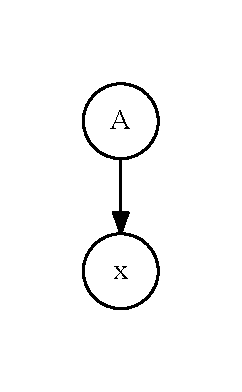
\includegraphics[width=0.2\textwidth]{pictures/tree1.pdf}
 \caption{The derivation tree of the height $h = 1$ for the string $x = l(\pi)$.}
 \label{tree1}
\end{figure}

\textbf{Inductive step}: Assume that the statement of the lemma holds for any $k \leq (p - 1)$ and show that it also holds for $k = p$ where $p \geq 2$. For any $i, j$ and for any non-terminal $A \in N$, $$A \in a^{(p)}_{i,j} \text{ iff } A \in a^{(p-1)}_{i,j} \text{ or } A \in (a^{(p-1)} \times a^{(p-1)})_{i,j},$$ since $$a^{(p)} = a^{(p-1)} \cup (a^{(p-1)} \times a^{(p-1)}).$$

Let $A \in a^{(p-1)}_{i,j}$. By the inductive hypothesis, $A \in a^{(p-1)}_{i,j}$ iff $(i,j) \in R_A$ and there exists $i \pi j$, such that there is a derivation tree of the height $h \leq (p-1)$ for the string $l(\pi)$ and a context-free grammar $G_A = (N,\Sigma,P,A)$. The statement of the lemma holds for $k = p$ since the height $h$ of this tree is also less than or equal to $p$.

Let $A \in (a^{(p-1)} \times a^{(p-1)})_{i,j}$. By the definition of the binary operation $(\cdot)$ on arbitrary subsets, $A \in (a^{(p-1)} \times a^{(p-1)})_{i,j}$ iff there are $r$, $B \in a^{(p-1)}_{i,r}$ and $C \in a^{(p-1)}_{r,j}$, such that $(A \rightarrow B C) \in P$. Hence, by the inductive hypothesis, there are $i \pi_1 r$ and $r \pi_2 j$, such that $(i,r) \in R_B$ and $(r,j) \in R_C$, and there are the derivation trees $T_B$ and $T_C$ of heights $h_1 \leq (p-1)$ and $h_2 \leq (p-1)$ for the strings $w_1 = l(\pi_1)$, $w_2 = l(\pi_2)$ and the context-free grammars $G_B$, $G_C$ respectively. Thus, the concatenation of paths $\pi_1$ and $\pi_2$ is $i \pi j$, where $(i,j) \in R_A$ and there is a derivation tree of the height $h = 1 + max(h_1, h_2)$, shown in Figure~\ref{tree2}, for the string $w = l(\pi)$ and a context-free grammar $G_A$.

\begin{figure}[h!]
 \centering
 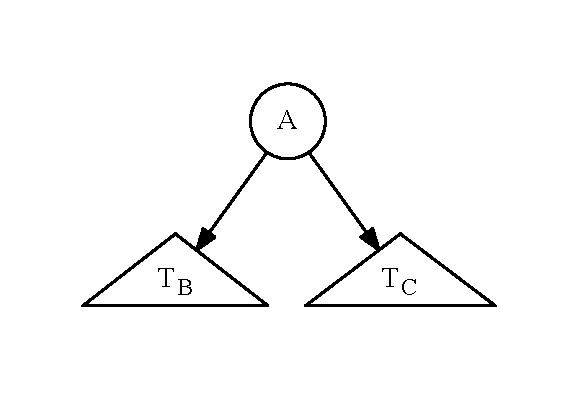
\includegraphics[width=0.8\textwidth]{pictures/tree2.pdf}
 \caption{The derivation tree of the height $h = 1 + max(h_1, h_2)$ for the string $w = l(\pi)$, where $T_B$ and $T_C$ are the derivation trees for strings $w_1$ and $w_2$ respectively.}
 \label{tree2}
\end{figure}

The statement of the lemma holds for $k = p$ since the height $h = 1 + max(h_1, h_2) \leq p$. This completes the proof of the lemma.
\end{proof}

\begin{mytheorem}\label{thm:correct}
 Let $D = (V,E)$ be a graph and let $G =(N,\Sigma,P)$ be a grammar. Then for any $i, j$ and for any non-terminal $A \in N$, $A \in a^{cf}_{i,j}$ iff $(i,j) \in R_A$.
\end{mytheorem}
\begin{proof}

Since the matrix $a^{cf} = a^{(1)} \cup a^{(2)} \cup \cdots,$ for any $i, j$ and for any non-terminal $A \in N$, $A \in a^{cf}_{i,j}$ iff there is $k \geq 1$, such that $A \in a^{(k)}_{i,j}$. By the lemma~\ref{lemma:cf}, $A \in a^{(k)}_{i,j}$ iff $(i,j) \in R_A$ and there is $i \pi j$, such that there is a derivation tree of the height $h \leq k$ for the string $l(\pi)$ and a context-free grammar $G_A = (N,\Sigma,P,A)$. This completes the proof of the theorem.
\end{proof}

We can, therefore, determine whether $(i,j) \in R_A$ by asking whether $A \in a^{cf}_{i,j}$. Thus, we show how the context-free relations $R_A$ can be calculated by computing the transitive closure $a^{cf}$ of the matrix $a$.



\subsection{The algorithm} \label{section_algorithm}
In this section, we introduce an algorithm for calculating the transitive closure $a^{cf}$ which was discussed in Section~\ref{section_reducing}.

Let $D = (V, E)$ be the input graph and $G = (N,\Sigma,P)$ be the input grammar.

\begin{algorithm}[H]
\begin{algorithmic}[1]
\caption{Context-free recognizer for graphs}
\label{alg:graphParse}
\Function{contextFreePathQuerying}{D, G}
    
    \State{$n \gets$ the number of nodes in $D$}
    \State{$E \gets$ the directed edge-relation from $D$}
    \State{$P \gets$ the set of production rules in $G$}
    \State{$T \gets$ the matrix $n \times n$ in which each element is $\varnothing$}
    \ForAll{$(i,x,j) \in E$}
    \Comment{Matrix initialization}
        \State{$T_{i,j} \gets T_{i,j} \cup \{A~|~(A \rightarrow x) \in P \}$}
    \EndFor    
    \While{matrix $T$ is changing}
       
        \State{$T \gets T \cup (T \times T)$}
        \Comment{Transitive closure $T^{cf}$ calculation} 
    \EndWhile
\State \Return $T$
\EndFunction
\end{algorithmic}
\end{algorithm}

Note that the matrix initialization in lines \textbf{6-7} of the Algorithm~\ref{alg:graphParse} can handle arbitrary graph $D$. For example, if a graph $D$ contains multiple edges $(i,x_1,j)$ and $(i,x_2,j)$ then both the elements of the set $\{A~|~(A \rightarrow x_1) \in P \}$ and the elements of the set $\{A~|~(A \rightarrow x_2) \in P \}$ will be added to $T_{i,j}$.

We need to show that the Algorithm~\ref{alg:graphParse} terminates in a finite number of steps. Since each element of the matrix $T$ contains no more than $|N|$ non-terminals, the total number of non-terminals in the matrix $T$ does not exceed $|V|^2|N|$. Therefore, the following theorem holds.

\begin{mytheorem}\label{thm:finite}
 Let $D = (V,E)$ be a graph and let $G =(N,\Sigma,P)$ be a grammar. The Algorithm~\ref{alg:graphParse} terminates in a finite number of steps. 
\end{mytheorem}
\begin{proof}
It is sufficient to show, that the operation in the line \textbf{9} of the Algorithm~\ref{alg:graphParse} changes the matrix $T$ only finite number of times. Since this operation can only add non-terminals to some elements of the matrix $T$, but not remove them, it can change the matrix $T$ no more than $|V|^2|N|$ times.
\end{proof}

Denote the number of elementary operations executed by the algorithm of multiplying two $n \times n$ Boolean matrices as $BMM(n)$. According to Valiant, the matrix multiplication operation in the line \textbf{9} of the Algorithm~\ref{alg:graphParse} can be calculated in $O(|N|^2 BMM(|V|))$. Denote the number of elementary operations executed by the matrix union operation of two $n \times n$ Boolean matrices as $BMU(n)$. Similarly, it can be shown that the matrix union operation in the line \textbf{9} of the Algorithm~\ref{alg:graphParse} can be calculated in $O(|N|^2 BMU(n))$. Since the line \textbf{9} of the Algorithm~\ref{alg:graphParse} is executed no more than $|V|^2|N|$ times, the following theorem holds.

\begin{mytheorem}\label{thm:time}
 Let $D = (V,E)$ be a graph and let $G =(N,\Sigma,P)$ be a grammar. The Algorithm~\ref{alg:graphParse} calculates the transitive closure $T^{cf}$ in $O(|V|^2|N|^3(BMM(|V|) + BMU(|V|)))$.
\end{mytheorem}

We also provide the worst-case example, for which the time complexity in terms of the graph size provided by Theorem~\ref{thm:time} cannot be improved. This example is based on the context-free grammar $G = (N, \Sigma, P)$ where:
\begin{itemize}
	\item the set of non-terminals $N = \{S\}$;
	\item the set of terminals $\Sigma = \{a, b\}$;
	\item the set of production rules $P$ is presented on Figure~\ref{ProductionRulesWorsCaseExample}.
\end{itemize}

\begin{figure}[h]
	\[
	\begin{array}{rccl}
	0: & S & \rightarrow & \text{\emph{a}} \ S \ \text{\emph{b}} \\
	1: & S & \rightarrow & \text{\emph{a}} \ \text{\emph{b}} \\ 
	\end{array}
	\]
	\caption{Production rules for the worst-case example.}
	\label{ProductionRulesWorsCaseExample}
\end{figure}

Let the size $|N|$ of the grammar $G$ be a constant. The worst-case time complexity is reached by running this query on the double-cyclic graph where:
\begin{itemize}
	\item one of the cycles having $u = 2^k + 1$ edges labeled with $a$;
	\item another cycle having $v = 2^k$ edges labeled with $b$;
	\item the two cycles are connected via a shared node $m$.
\end{itemize}

A small example of such graph with $k = 1$, $u = 3$, $v = 2$, and $m = 0$ is presented on Figure~\ref{worst_case_graph}.

\begin{figure}[h]
	\[
	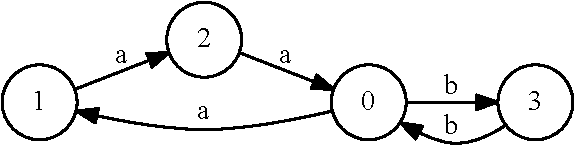
\includegraphics[width=0.8\textwidth]{pictures/worst_case_graph.pdf}
	\]
	\caption{An example of the graph for the worst-case time complexity.}
	\label{worst_case_graph}
\end{figure}

The shortest path $\pi$ from the node $m$ to the node $m$, whose labeling forms a string from the language $L(G_S)=\{a^n b^n; n \geq 1\}$, has a length $l = 2*u*v$, since $u = 2^k + 1$ and $v = 2^k$ are coprime, and string $s$, formed by this path, consists of $u*v$ labels $a$ and $u*v$ labels $b$. The string $s = l(\pi)$ has a derivation tree according to a context-free grammar $G_S$ of the minimal height $h = 2*u*v$ among all the paths from the node $m$ to the node $m$ in this double-cyclic graph. Therefore, if we run the worst-case example query on this graph, then the operation in the line \textbf{9} of the Algorithm~\ref{alg:graphParse} changes the matrix $T$ at least $h = 2*u*v$ times. Hence, the Algorithm~\ref{alg:graphParse} computes this query in $O(|V|^2(BMM(|V|) + BMU(|V|)))$, since $|V| = (u + v - 1) = 2*v$ and $h = 2*u*v > 2*v*v = |V|^2 / 4 = O(|V|^2)$.


\subsection{An example} \label{section_example}
In this section, we provide a step-by-step demonstration of the proposed algorithm. For this, we consider the classical \textit{same-generation query}~\cite{FndDB}.

The \textbf{example query} is based on the context-free grammar $G = (N, \Sigma, P)$ where:
\begin{itemize}
    \item The set of non-terminals $N = \{S\}$.
    \item The set of terminals $$\Sigma = \{subClassOf, subClassOf^{-1}, type, type^{-1}\}.$$
    \item The set of production rules $P$ is presented in Figure~\ref{ProductionRulesExampleQuery}.
\end{itemize}

\begin{figure}[h]
   \[
\begin{array}{rccl}
   0: & S & \rightarrow & \text{\textit{subClassOf}}^{-1} \ S \ \text{\textit{subClassOf}} \\ 
   1: & S & \rightarrow & \text{\textit{type}}^{-1} \ S \ \text{\textit{type}} \\ 
   2: & S & \rightarrow & \text{\textit{subClassOf}}^{-1} \ \text{\textit{subClassOf}} \\ 
   3: & S & \rightarrow & \text{\textit{type}}^{-1} \ \text{\textit{type}} \\ 
\end{array}
\]
\caption{Production rules for the example query grammar.}
\label{ProductionRulesExampleQuery}
\end{figure}

Since the proposed algorithm processes only grammars in Chomsky normal form, we first transform the grammar $G$ into an equivalent grammar $G' = (N', \Sigma', P')$ in normal form, where:
\begin{itemize}
    \item The set of non-terminals $N' = \{S, S_1, S_2, S_3, S_4, S_5, S_6\}$.
    \item The set of terminals $$\Sigma' = \{subClassOf, subClassOf^{-1}, type, type^{-1}\}.$$
    \item The set of production rules $P'$ is presented in Figure~\ref{ProductionRulesExampleQueryCNF}.
\end{itemize}

\begin{figure}[h]
   \[
\begin{array}{rccl}
   0: & S & \rightarrow & S_1 \ S_5 \\
   1: & S & \rightarrow & S_3 \ S_6 \\
   2: & S & \rightarrow & S_1 \ S_2 \\
   3: & S & \rightarrow & S_3 \ S_4 \\
   4: & S_5 & \rightarrow & S \ S_2 \\
   5: & S_6 & \rightarrow & S \ S_4 \\
   6: & S_1 & \rightarrow & \text{\textit{subClassOf}}^{-1} \\ 
   7: & S_2 & \rightarrow & \text{\textit{subClassOf}} \\ 
   8: & S_3 & \rightarrow & \text{\textit{type}}^{-1} \\
   9: & S_4 & \rightarrow & \text{\textit{type}} \\ 
\end{array}
\]
\caption{Production rules for the example query grammar in normal form.}
\label{ProductionRulesExampleQueryCNF}
\end{figure}

We run the query on a graph presented in Figure~\ref{ExampleQueryGraph}.

\begin{figure}[h]
\[
    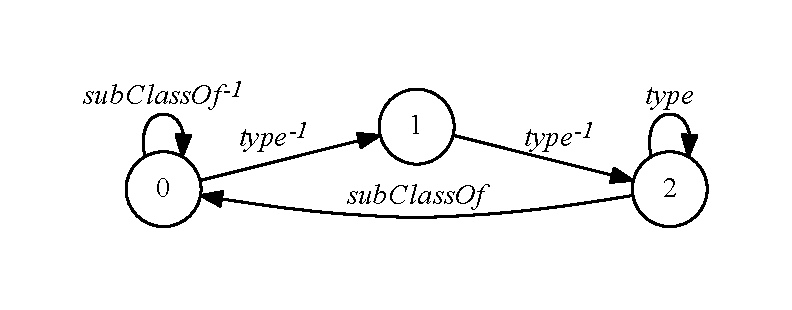
\includegraphics[width=0.8\textwidth]{pictures/ExampleGraph.pdf}
\]
\caption{An input graph for the example query.}
\label{ExampleQueryGraph}
\end{figure}

We provide a step-by-step demonstration of the work with the given graph $D$ and grammar $G'$ of the Algorithm~\ref{alg:graphParse}. After the matrix initialization in lines \textbf{6-7} of the Algorithm~\ref{alg:graphParse}, we have a matrix $T_0$ presented in Figure~\ref{ExampleQueryInitMatrix}.

\begin{figure}[h]
\[
T_0 = \begin{pmatrix}
    \{S_1\} & \{S_3\} & \varnothing \\ \varnothing & \varnothing & \{S_3\} \\ \{S_2\} & \varnothing & \{S_4\}
\end{pmatrix}
\]
\caption{The initial matrix for the example query.}
\label{ExampleQueryInitMatrix}
\end{figure}

Let $T_i$ be the matrix $T$ obtained after executing the loop in lines \textbf{8-9} of the Algorithm~\ref{alg:graphParse} $i$ times. The calculation of the matrix $T_1$ is shown in Figure~\ref{ExampleQueryFirstIteration}.

\begin{figure}[h]
\[
T_0 \times T_0 = \begin{pmatrix}
    \varnothing & \varnothing & \varnothing \\ \varnothing & \varnothing & \{S\} \\ \varnothing & \varnothing & \varnothing
\end{pmatrix}
\]

\[
T_1 = T_0 \cup (T_0 \times T_0) = \begin{pmatrix}
    \{S_1\} & \{S_3\} & \varnothing \\ \varnothing & \varnothing & \{S_3, S\} \\ \{S_2\} & \varnothing & \{S_4\}
\end{pmatrix}
\]
\caption{The first iteration of computing the transitive closure for the example query.}
\label{ExampleQueryFirstIteration}
\end{figure}

When the algorithm at some iteration finds new paths in the graph $D$, then it adds corresponding nonterminals to the matrix $T$. For example, after the first loop iteration, non-terminal $S$ is added to the matrix $T$. This non-terminal is added to the element with a row index $i = 1$ and a column index $j = 2$. This means that there is $i\pi j$ (a path $\pi$ from the node 1 to the node 2), such that $S \xrightarrow{*} l(\pi)$. For example, such a path consists of two edges with labels $type^{-1}$ and $type$, and thus $S \xrightarrow{*} type^{-1} \ type$.

The calculation of the transitive closure is completed after $k$ iterations when a fixpoint is reached: $T_{k-1} = T_k$. For the example query, $k = 6$ since $T_6 = T_5$. The remaining iterations of computing the transitive closure are presented in Figure~\ref{ExampleQueryFinalIterations}.

\begin{figure}[h]
\[
T_2 = \begin{pmatrix}
    \{S_1\} & \{S_3\} & \varnothing \\ \{S_5\} & \varnothing & \{S_3, S, S_6\} \\ \{S_2\} & \varnothing & \{S_4\}
\end{pmatrix}
\]

\[
T_3 = \begin{pmatrix}
    \{S_1\} & \{S_3\} & \{S\} \\ \{S_5\} & \varnothing & \{S_3, S, S_6\} \\ \{S_2\} & \varnothing & \{S_4\}
\end{pmatrix}
\]

\[
T_4 = \begin{pmatrix}
    \{S_1, S_5\} & \{S_3\} & \{S, S_6\} \\ \{S_5\} & \varnothing & \{S_3, S, S_6\} \\ \{S_2\} & \varnothing & \{S_4\}
\end{pmatrix}
\]

\[
T_5 = \begin{pmatrix}
    \{S_1, S_5, S\} & \{S_3\} & \{S, S_6\} \\ \{S_5\} & \varnothing & \{S_3, S, S_6\} \\ \{S_2\} & \varnothing & \{S_4\}
\end{pmatrix}
\]
\caption{Remaining states of the matrix $T$.}
\label{ExampleQueryFinalIterations}
\end{figure}

Thus, the result of the Algorithm~\ref{alg:graphParse} for the example query is the matrix $T_5 = T_6$. Now, after constructing the transitive closure, we can construct the context-free relations $R_A$. These relations for each non-terminal of the grammar $G'$ are presented in Figure~\ref{ExampleQueryCFRelations}.

\begin{figure}[h]
\begin{eqnarray*}
R_S&=&\{(0,0),(0,2),(1,2)\},\\
R_{S_1}&=&\{(0,0)\},\\
R_{S_2}&=&\{(2,0)\}, \\
R_{S_3}&=&\{(0,1), (1,2)\}, \\
R_{S_4}&=&\{(2,2)\}, \\
R_{S_5}&=&\{(0,0), (1,0)\}, \\
R_{S_6}&=&\{(0,2), (1,2)\}.
\end{eqnarray*}
\caption{Context-free relations for the example query.}
\label{ExampleQueryCFRelations}
\end{figure}

By the context-free relation $R_S$, we can conclude that there are paths in a graph $D$ only from the node 0 to the node 0, from the node 0 to the node 2 or from the node 1 to the node 2, corresponding to the context-free grammar $G_S$. This conclusion is based on the fact that a grammar $G'_S$ is equivalent to the grammar $G_S$ and $L(G_S) = L(G_S')$.

\section{CFPQ using single-path query semantics}
In this section, we show how the context-free path query evaluation using the single-path query semantics can be reduced to the calculation of matrix transitive closure $a^{cf}$ and prove the correctness of this reduction.

At the first step, we show how the calculation of matrix transitive closure $a^{cf}$ which was discussed in Section~\ref{section_reducing} can be modified to compute the length of some path $i \pi j$ for all $(i,j) \in R_A$, such that $A \xrightarrow{*} l(\pi)$. This is sufficient to solve the problem of context-free path query evaluation using the single-path query semantics since the required path of a fixed length from the node $i$ to the node $j$ can be found by a simple search and checking whether the labels of this path form a string which can be derived from a non-terminal $A$.

Let $G = (N,\Sigma,P)$ be a grammar and $D = (V, E)$ be a graph. We enumerate the nodes of the graph $D$ from 0 to $(|V| - 1)$. We initialize the $|V| \times |V|$ matrix $a$ with $\varnothing$. We associate each non-terminal in matrix $a$ with the corresponding path length. For convenience, each nonterminal $A$ in the $a_{i,j}$ is represented as a pair $(A,k)$ where $k$ is an associated path length. For every $i$ and $j$ we set $$a_{i,j} = \{(A_k,1)~|~((i,x,j) \in E) \wedge ((A_k \rightarrow x) \in P)\}$$ since initially all path lengths are equal to $1$. Finally, we compute the transitive closure $a^{cf}$ and if non-terminal $A$ is added to $a^{(p)}_{i,j}$ by using the production rule $(A \rightarrow B C) \in P$ where $(B,l_B) \in a^{(p-1)}_{i,k}$, $(C,l_C) \in a^{(p-1)}_{k,j}$, then the path length $l_A$ associated with non-terminal $A$ is calculated as $l_A = l_B + l_C$. Therefore $(A, l_A) \in a^{(p)}_{i,j}$. Note that if some non-terminal $A$ with an associated path length $l_1$ is in $a^{(p)}_{i,j}$, then the non-terminal $A$ is not added to the $a^{(k)}_{i,j}$ with an associated path length $l_2$ for all $l_2 \neq l_1$ and $k \geq p$. For the transitive closure $a^{cf}$, the following statements hold.

\begin{lemma}\label{lemma:singlepath}
	Let $D = (V,E)$ be a graph, let $G =(N,\Sigma,P)$ be a grammar. Then for any $i, j$ and for any non-terminal $A \in N$, if $(A,l_A) \in a^{(k)}_{i,j}$, then there is $i \pi j$, such that $A \xrightarrow{*} l(\pi)$ and the length of $\pi$ is equal to $l_A$.
\end{lemma}
\begin{proof}(Proof by Induction)
	
	\textbf{Basis}: Show that the statement of the lemma holds for $k = 1$. For any $i, j$ and for any non-terminal $A \in N$, $(A, l_A) \in a^{(1)}_{i,j}$ iff $l_A = 1$ and there is $i \pi j$ that consists of a unique edge $e$ from the node $i$ to the node $j$ and $(A \rightarrow x) \in P$ where $x = l(\pi)$. Therefore there is $i \pi j$, such that $A \xrightarrow{*} l(\pi)$ and the length of $\pi$ is equal to $l_A$. Thus, it has been shown that the statement of the lemma holds for $k = 1$.
	
	\textbf{Inductive step}: Assume that the statement of the lemma holds for any $k \leq (p - 1)$ and show that it also holds for $k = p$ where $p \geq 2$. For any $i, j$ and for any non-terminal $A \in N$, $(A, l_A) \in a^{(p)}_{i,j}$ iff $(A, l_A) \in a^{(p-1)}_{i,j}$ or $(A, l_A) \in (a^{(p-1)} \times a^{(p-1)})_{i,j}$ since $a^{(p)} = a^{(p-1)} \cup (a^{(p-1)} \times a^{(p-1)}).$
	
	Let $(A, l_A) \in a^{(p-1)}_{i,j}$. By the inductive hypothesis, there is $i \pi j$, such that $A \xrightarrow{*} l(\pi)$ and the length of $\pi$ is equal to $l_A$. Therefore the statement of the lemma holds for $k = p$.
	
	Let $(A, l_A) \in (a^{(p-1)} \times a^{(p-1)})_{i,j}$. By the definition, $(A, l_A) \in (a^{(p-1)} \times a^{(p-1)})_{i,j}$ iff there are $r$, $(B, l_B) \in a^{(p-1)}_{i,r}$ and $(C, l_C) \in a^{(p-1)}_{r,j}$, such that $(A \rightarrow B C) \in P$ and $l_A = l_B + l_C$. Hence, by the inductive hypothesis, there are $i \pi_1 r$ and $r \pi_2 j$, such that $$(B \xrightarrow{*} l(\pi_1)) \wedge(C \xrightarrow{*} l(\pi_2)),$$ where the length of $\pi_1$ is equal to $l_B$ and the length of $\pi_2$ is equal to $l_C$. Thus, the concatenation of paths $\pi_1$ and $\pi_2$ is $i \pi j$, where $A \xrightarrow{*} l(\pi)$ and the length of $\pi$ is equal to $l_A$. Therefore the statement of the lemma holds for $k = p$ and this completes the proof of the lemma.
\end{proof}

\begin{mytheorem}\label{thm:singlepathcorrect}
	Let $D = (V,E)$ be a graph and let $G =(N,\Sigma,P)$ be a grammar. Then for any $i, j$ and for any non-terminal $A \in N$, if $(A, l_A) \in a^{cf}_{i,j}$, then there is $i \pi j$, such that $A \xrightarrow{*} l(\pi)$ and the length of $\pi$ is equal to $l_A$.
\end{mytheorem}
\begin{proof}
	
	Since the matrix $a^{cf} = a^{(1)} \cup a^{(2)} \cup \cdots$, for any $i, j$ and for any non-terminal $A \in N$, if $(A, l_A) \in a^{cf}_{i,j}$, then there is $k \geq 1$, such that $A \in a^{(k)}_{i,j}$. By the lemma~\ref{lemma:singlepath}, if $(A, l_A) \in a^{(k)}_{i,j}$, then there is $i \pi j$, such that $A \xrightarrow{*} l(\pi)$ and the length of $\pi$ is equal to $l_A$. This completes the proof of the theorem.
\end{proof}

By the theorem~\ref{thm:correct}, we can determine whether $(i,j) \in R_A$ by asking whether $(A, l_A) \in a^{cf}_{i,j}$ for some $l_A$. By the theorem~\ref{thm:singlepathcorrect}, there is $i \pi j$, such that $A \xrightarrow{*} l(\pi)$ and the length of $\pi$ is equal to $l_A$. Therefore, we can find such a path $\pi$ of the length $l_A$ from the node $i$ to the node $j$ by a simple search. Thus, we show how the context-free path query evaluation using the single-path query semantics can be reduced to the calculation of matrix transitive closure $a^{cf}$. Note that the time complexity of the algorithm for context-free path querying w.r.t. the single-path semantics no longer depends on the Boolean matrix multiplications since we modify the matrix representation and operations on the matrix elements.

\section{A path querying algorithm using conjunctive grammars}
In this section, we show how the path querying using conjunctive grammars and relational query semantics can be reduced to the calculation of the matrix transitive closure. We propose an algorithm that calculates the over-approximation of all conjunctive relations $R_A$, since the query evaluation using the relational query semantics and conjunctive grammars is undecidable problem~\cite{hellingsRelational}.

We define a \textit{conjunctive matrix multiplication}, $a \circ b = c$, where $a$ and $b$ are matrices of the suitable size that have subsets of $N$ as elements, as $c_{i,j} = \{A~|~\exists (A \rightarrow B_1 C_1~\& \ldots \&~B_m C_m) \in P \text{ such that } (B_k, C_k) \in d_{i,j} \}$, where $d_{i,j} = \bigcup^{n}_{k=1}{a_{i,k} \times b_{k,j}}$ and $(\times)$ is the Cartesian product. 

We define the \textit{conjunctive transitive closure} of a square matrix $a$ as $a^{conj} = a^{(1)} \cup a^{(2)} \cup \cdots$ where $a^{(i)} = a^{(i-1)} \cup (a^{(i-1)} \circ a^{(i-1)})$, $i \ge 2$ and $a^{(1)} = a$.

\subsection{Reducing conjunctive path querying to transitive closure} \label{section_reducing_conj}
In this section, we show how the over-approximation of all conjunctive relations $R_A$ can be calculated by computing the transitive closure $a^{conj}$.

Let $G = (N,\Sigma,P)$ be a conjunctive grammar and $D = (V, E)$ be a graph. We number the nodes of the graph $D$ from 0 to $(|V| - 1)$ and we associate the nodes with their numbers. We initialize $|V| \times |V|$ matrix $b$ with $\emptyset$. Further, for every $i$ and $j$ we set $b_{i,j} = \{A_k~|~((i,x,j) \in E) \wedge ((A_k \rightarrow x) \in P)\}$. Finally, we compute the conjunctive transitive closure $b^{conj} = b^{(1)} \cup b^{(2)} \cup \cdots$ where $b^{(i)} = b^{(i-1)} \cup (b^{(i-1)} \circ b^{(i-1)})$, $i \ge 2$ and $b^{(1)} = b$. For the conjunctive transitive closure $b^{conj}$, the following statements holds.

\begin{lemma}\label{lemma:conj}
	Let $D = (V,E)$ be a graph, let $G =(N,\Sigma,P)$ be a conjunctive grammar. Then for any $i, j$ and for any non-terminal $A \in N$, if $(i,j) \in R_A$ and $i \pi j$, such that there is a derivation tree according to the string $l(\pi)$ and a conjunctive grammar $G_A = (N,\Sigma,P,A)$ of the height $h \leq k$ then $A \in b^{(k)}_{i,j}$.
\end{lemma}
\begin{proof}(Proof by Induction)
	
	\textbf{Basis}: Show that the statement of the lemma holds for $k = 1$. For any $i, j$ and for any non-terminal $A \in N$, if $(i,j) \in R_A$ and $i \pi j$, such that there is a derivation tree according to the string $l(\pi)$ and a conjunctive grammar $G_A = (N,\Sigma,P,A)$ of the height $h \leq 1$ then there is edge $e$ from node $i$ to node $j$ and $(A \rightarrow x) \in P$ where $x = l(\pi)$. Therefore $A \in b^{(1)}_{i,j}$ and it has been shown that the statement of the lemma holds for $k = 1$.
	
	\textbf{Inductive step}: Assume that the statement of the lemma holds for any $k \leq (p - 1)$ and show that it also holds for $k = p$ where $p \geq 2$. Let $(i,j) \in R_A$ and $i \pi j$, such that there is a derivation tree according to the string $l(\pi)$ and a conjunctive grammar $G_A = (N,\Sigma,P,A)$ of the height $h \leq p$.
	
	Let $h < p$. Then by the inductive hypothesis $A \in b^{(p-1)}_{i,j}$. Since $b^{(p)} = b^{(p-1)} \cup (b^{(p-1)} \circ b^{(p-1)})$ then $A \in b^{(p)}_{i,j}$ and the statement of the lemma holds for $k = p$.
	
	Let $h = p$. Let $A \rightarrow B_1 C_1~\& \ldots \&~B_m C_m$ be the rule corresponding to the root of the derivation tree from the assumption of the lemma. Therefore the heights of all subtrees corresponding to non-terminals $B_1, C_1, \ldots B_m, C_m$ are less than $p$. Then by the inductive hypothesis $B_x \in b^{(p-1)}_{i,t_x}$ and $C_x \in b^{(p-1)}_{t_x,j}$, for $x = 1\ldots m$ and $t_x \in V$. Let $d$ be a matrix that have subsets of $N \times N$ as elements, where $d_{i,j} = \bigcup^{n}_{t=1}{b^{(p-1)}_{i,t} \times b^{(p-1)}_{t,j}}$. Therefore $(B_x, C_x) \in d_{i,j}$, for $x = 1\ldots m$. Since $b^{(p)} = b^{(p-1)} \cup (b^{(p-1)} \circ b^{(p-1)})$ and $(b^{(p-1)} \circ b^{(p-1)})_{i,j} = \{A~|~\exists (A \rightarrow B_1 C_1~\& \ldots \&~B_m C_m) \in P \text{ such that } (B_k, C_k) \in d_{i,j} \}$ then $A \in b^{(p)}_{i,j}$ and the statement of the lemma holds for $k = p$. This completes the proof of the lemma.
\end{proof}

\begin{mytheorem}\label{thm:correct_conj}
	Let $D = (V,E)$ be a graph and let $G =(N,\Sigma,P)$ be a conjunctive grammar. Then for any $i, j$ and for any non-terminal $A \in N$, if $(i,j) \in R_A$ then $A \in b^{conj}_{i,j}$.
\end{mytheorem}
\begin{proof}
	
	By the lemma~\ref{lemma:conj}, if $(i,j) \in R_A$ then $A \in b^{(k)}_{i,j}$ for some $k$, such that $i \pi j$ with a derivation tree according to the string $l(\pi)$ and a conjunctive grammar $G_A = (N,\Sigma,P,A)$ of the height $h \leq k$. Since the matrix $b^{conj} = b^{(1)} \cup b^{(2)} \cup \cdots$, then for any $i, j$ and for any non-terminal $A \in N$, if $A \in b^{(k)}_{i,j}$ for some $k \geq 1$ then  $A \in b^{conj}_{i,j}$. Therefore, if $(i,j) \in R_A$ then $A \in b^{conj}_{i,j}$. This completes the proof of the theorem.
\end{proof}

Thus, we show how the over-approximation of all conjunctive relations $R_A$ can be calculated by computing the conjunctive transitive closure $b^{conj}$ of the matrix $b$.



\subsection{The algorithm} \label{section_algorithm_conj}
In this section we introduce an algorithm for calculating the conjunctive transitive closure $b^{conj}$ which was discussed in Section~\ref{section_reducing_conj}.

The following algorithm takes on input a graph $D = (V, E)$ and a conjunctive grammar $G = (N,\Sigma,P)$.

\begin{algorithm}[H]
	\begin{algorithmic}[1]
		\caption{Conjunctive recognizer for graphs}
		\label{alg:graphParse_conj}
		\Function{conjunctiveGraphParsing}{D, G}
		
		\State{$n \gets$ a number of nodes in $D$}
		\State{$E \gets$ the directed edge-relation from $D$}
		\State{$P \gets$ a set of production rules in $G$}
		\State{$T \gets$ a matrix $n \times n$ in which each element is $\emptyset$}
		\ForAll{$(i,x,j) \in E$}
		\Comment{Matrix initialization}
		\State{$T_{i,j} \gets T_{i,j} \cup \{A~|~(A \rightarrow x) \in P \}$}
		\EndFor    
		\While{matrix $T$ is changing}
		
		\State{$T \gets T \cup (T \circ T)$}
		\Comment{Transitive closure calculation} 
		\EndWhile
		\State \Return $T$    
		\EndFunction
	\end{algorithmic}
\end{algorithm}

Similar to the case of the context-free grammars we can show that the Algorithm~\ref{alg:graphParse_conj} terminates in a finite number of steps. Since each element of the matrix $T$ contains no more than $|N|$ non-terminals, then total number of non-terminals in the matrix $T$ does not exceed $|V|^2|N|$. Therefore, the following theorem holds.

\begin{mytheorem}\label{thm:finite_conj}
	Let $D = (V,E)$ be a graph and let $G =(N,\Sigma,P)$ be a conjunctive grammar. Algorithm~\ref{alg:graphParse_conj} terminates in a finite number of steps. 
\end{mytheorem}
\begin{proof}
	It is sufficient to show, that the operation in line \textbf{9} of the Algorithm~\ref{alg:graphParse_conj} changes the matrix $T$ only finite number of times. Since this operation can only add non-terminals to some elements of the matrix $T$, but not remove them, it can change the matrix $T$ no more than $|V|^2|N|$ times.
\end{proof}

\subsection{An example}
In this section, we provide a step-by-step demonstration of the proposed algorithm for path querying using conjunctive grammars. The \textbf{example query} is based on the conjunctive grammar $G = (N, \Sigma, P)$ in binary normal form where:
\begin{itemize}
	\item The set of non-terminals $N = \{S, A, B, C, D\}$.
	\item The set of terminals $\Sigma = \{a, b, c\}.$
	\item The set of production rules $P$ is presented in Figure~\ref{ProductionRulesExampleQueryConj}.
\end{itemize}

\begin{figure}[h]
	\[
	\begin{array}{rccl}
	0: & S & \rightarrow & AB \ \& \ DC \\ 
	1: & A & \rightarrow & a \\ 
	2: & B & \rightarrow & BC \\ 
	3: & B & \rightarrow & b \\
	4: & C & \rightarrow & c \\ 
	5: & D & \rightarrow & AD \\ 
	6: & D & \rightarrow & b \\ 
	\end{array}
	\]
	\caption{Production rules for the conjunctive example query grammar.}
	\label{ProductionRulesExampleQueryConj}
\end{figure}

The conjunct $AB$ generates the language $L_{AB} = \{abc^*\}$ and the conjunct $DC$ generates the language $L_{DC} = \{a^*bc\}$. Thus, the language generated by the conjunctive grammar $G_S = (N, \Sigma, P, S)$ is $L(G_S) = L_{AB} \cap L_{DC} = \{abc\}$. We tun the query on a graph presented in Figure~\ref{conjExampleGraph}.

\begin{figure}[h]
	\[
	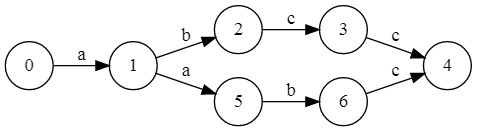
\includegraphics[width=0.8\textwidth]{pictures/ConjExampleGraph.png}
	\]
	\caption{An input graph for the conjunctive example query.}
	\label{conjExampleGraph}
\end{figure}

We provide a step-by-step demonstration of the work with the given graph $D$ and grammar $G$ of the Algorithm~\ref{alg:graphParse_conj}. After the matrix initialization in lines \textbf{6-7} of the Algorithm~\ref{alg:graphParse_conj}, we have a matrix $T_0$ presented in Figure~\ref{ConjExampleQueryInitMatrix}.

\begin{figure}[h]
	\[
	T_0 = \begin{pmatrix}
	\varnothing & \{A\} & \varnothing & \varnothing & \varnothing & \varnothing & \varnothing \\
	
	\varnothing & \varnothing & \{B, D\} & \varnothing & \varnothing & \{A\} & \varnothing \\
	
	\varnothing & \varnothing & \varnothing & \{C\} & \varnothing & \varnothing & \varnothing \\
	
	\varnothing & \varnothing & \varnothing & \varnothing & \{C\} & \varnothing & \varnothing \\
	
	\varnothing & \varnothing & \varnothing & \varnothing & \varnothing & \varnothing & \varnothing \\
	
	\varnothing & \varnothing & \varnothing & \varnothing & \varnothing & \varnothing & \{B, D\} \\
	
	\varnothing & \varnothing & \varnothing & \varnothing & \{C\} & \varnothing & \varnothing \\
	\end{pmatrix}
	\]
	\caption{The initial matrix for the example query.}
	\label{ConjExampleQueryInitMatrix}
\end{figure}

Let $T_i$ be the matrix $T$ obtained after executing the loop in lines \textbf{8-9} of the Algorithm~\ref{alg:graphParse_conj} $i$ times. To compute the matrix $T_1$ we need to compute the matrix $d$ where $d_{i,j} = \bigcup^{n}_{k=1}{T_{0_{i,k}} \times T_{0_{i,k}}}$. The matrix $d$ for the first loop iteration is presented in Figure~\ref{dmatrix}. The matrix $T_1 = $ $T_1 = T_0 \cup (T_0 \circ T_0)$ is shown in Figure~\ref{ConjExampleQueryFirstIteration}.

\begin{figure}[h]
	\noindent
	\resizebox{\linewidth}{!}{%
	$
	\begin{pmatrix}
	\varnothing & \varnothing & \{(A,B), (A,D)\} & \varnothing & \varnothing & \varnothing & \varnothing \\
	
	\varnothing & \varnothing & \varnothing & \{(B,C), (D,C)\} & \varnothing & \varnothing & \{(A,B), (A,D)\} \\
	
	\varnothing & \varnothing & \varnothing & \varnothing & \{(C,C)\} & \varnothing & \varnothing \\
	
	\varnothing & \varnothing & \varnothing & \varnothing & \varnothing & \varnothing & \varnothing \\
	
	\varnothing & \varnothing & \varnothing & \varnothing & \varnothing & \varnothing & \varnothing \\
	
	\varnothing & \varnothing & \varnothing & \varnothing & \{(B,C), (D,C)\} & \varnothing & \varnothing \\
	
	\varnothing & \varnothing & \varnothing & \varnothing & \varnothing & \varnothing & \varnothing \\
	\end{pmatrix}$%
	}
	\caption{The matrix $d$ for the first loop iteration.}
	\label{dmatrix}
\end{figure}

\begin{figure}[h]
	\[
	T_1 = \begin{pmatrix}
	\varnothing & \{A\} & \{D\} & \varnothing & \varnothing & \varnothing & \varnothing \\
	
	\varnothing & \varnothing & \{B, D\} & \{B\} & \varnothing & \{A\} & \{D\} \\
	
	\varnothing & \varnothing & \varnothing & \{C\} & \varnothing & \varnothing & \varnothing \\
	
	\varnothing & \varnothing & \varnothing & \varnothing & \{C\} & \varnothing & \varnothing \\
	
	\varnothing & \varnothing & \varnothing & \varnothing & \varnothing & \varnothing & \varnothing \\
	
	\varnothing & \varnothing & \varnothing & \varnothing & \{B\} & \varnothing & \{B, D\} \\
	
	\varnothing & \varnothing & \varnothing & \varnothing & \{C\} & \varnothing & \varnothing \\
	\end{pmatrix}
	\]
	\caption{The initial matrix for the example query.}
	\label{ConjExampleQueryFirstIteration}
\end{figure}

When the algorithm at some iteration finds new paths from the node $i$ to the node $j$ for all conjuncts of some production rule, then it adds nonterminal from the left side of this rule to the set $T_{i,j}$.

The calculation of the transitive closure is completed after $k$ iterations when a fixpoint is reached: $T_{k-1} = T_k$. For this example, $k = 4$ since $T_4 = T_3$. The remaining iterations of computing the transitive closure are presented in Figure~\ref{ConjExampleQueryFinalIterations}.

\begin{figure}
	\[
	T_2 = \begin{pmatrix}
	\varnothing & \{A\} & \{D\} & \{S\} & \varnothing & \varnothing & \{D\} \\
	
	\varnothing & \varnothing & \{B, D\} & \{B\} & \{S,B\} & \{A\} & \{D\} \\
	
	\varnothing & \varnothing & \varnothing & \{C\} & \varnothing & \varnothing & \varnothing \\
	
	\varnothing & \varnothing & \varnothing & \varnothing & \{C\} & \varnothing & \varnothing \\
	
	\varnothing & \varnothing & \varnothing & \varnothing & \varnothing & \varnothing & \varnothing \\
	
	\varnothing & \varnothing & \varnothing & \varnothing & \{B\} & \varnothing & \{B, D\} \\
	
	\varnothing & \varnothing & \varnothing & \varnothing & \{C\} & \varnothing & \varnothing \\
	\end{pmatrix}
	\]
	
	\[
	T_3 = \begin{pmatrix}
	\varnothing & \{A\} & \{D\} & \{S\} & \{S\} & \varnothing & \{D\} \\
	
	\varnothing & \varnothing & \{B, D\} & \{B\} & \{S,B\} & \{A\} & \{D\} \\
	
	\varnothing & \varnothing & \varnothing & \{C\} & \varnothing & \varnothing & \varnothing \\
	
	\varnothing & \varnothing & \varnothing & \varnothing & \{C\} & \varnothing & \varnothing \\
	
	\varnothing & \varnothing & \varnothing & \varnothing & \varnothing & \varnothing & \varnothing \\
	
	\varnothing & \varnothing & \varnothing & \varnothing & \{B\} & \varnothing & \{B, D\} \\
	
	\varnothing & \varnothing & \varnothing & \varnothing & \{C\} & \varnothing & \varnothing \\
	\end{pmatrix}
	\]
	
	\[
	T_4 = \begin{pmatrix}
	\varnothing & \{A\} & \{D\} & \{S\} & \{S\} & \varnothing & \{D\} \\
	
	\varnothing & \varnothing & \{B, D\} & \{B\} & \{S,B\} & \{A\} & \{D\} \\
	
	\varnothing & \varnothing & \varnothing & \{C\} & \varnothing & \varnothing & \varnothing \\
	
	\varnothing & \varnothing & \varnothing & \varnothing & \{C\} & \varnothing & \varnothing \\
	
	\varnothing & \varnothing & \varnothing & \varnothing & \varnothing & \varnothing & \varnothing \\
	
	\varnothing & \varnothing & \varnothing & \varnothing & \{B\} & \varnothing & \{B, D\} \\
	
	\varnothing & \varnothing & \varnothing & \varnothing & \{C\} & \varnothing & \varnothing \\
	\end{pmatrix}
	\]
	\caption{Remaining states of the matrix $T$.}
	\label{ConjExampleQueryFinalIterations}
\end{figure}

Thus, the result of the Algorithm~\ref{alg:graphParse_conj} for the example query is the matrix $T_4 = T_3$. Now, after constructing the transitive closure, we can construct the over-approximations $R'_A$ of the conjunctive relations $R_A$. These approximations for each non-terminal of the grammar $G$ are presented in Figure~\ref{ConjExampleQueryCFRelations}.

\begin{figure}
	\begin{eqnarray}
		R'_S&=&\{(0,3),(0,4),(1,4)\},\\
		R'_{A}&=&\{(0,1),(1,5)\},\\
		R'_{B}&=&\{(1,2),(1,3),(1,4),(5,4),(5,6)\}, \\
		R'_{C}&=&\{(2,3),(3,4),(6,4)\}, \\
		R'_{D}&=&\{(0,2),(0,6),(1,2),(1,6),(5,6)\}.
	\end{eqnarray}
	\caption{The over-approximations of the conjunctive relations for the example query.}
	\label{ConjExampleQueryCFRelations}
\end{figure}

This example demonstrates that it is not always possible to obtain an exact solution. For example, a pair of nodes $(0,4)$ belongs to $R'_S$, although there is no path from the node $0$ to the node $4$, which forms a string derived from the nonterminal $S$ (only the string $abc$ can be derived from the nonterminal $S$). Extra pairs of nodes are added if there are different paths from the node $i$ to the node $j$, which in summary correspond to all conjuncts of one production rule, but there is no path from the node $i$ to the node $j$, which at the same time would correspond to all conjuncts of this rule. For example, for the conjuncts of the rule $S \rightarrow AB \ \& \ DC$, there is a path from the node $0$ to the node $4$ forming the string $abcc$, and there is also a path from the node $0$ to the node $4$ forming the string $aabc$. The first path corresponds to the conjunct $AB$, since the string $abcc$ belongs to the language $L_{AB} = \{abc^*\}$, and the second path corresponds to the conjunct $DC$, since the string $aabc$ belongs to the language $L_{DC} = \{a^*bc\}$. However, it is obvious that there is no path from the node $0$ to the node $4$, which forms the string $abc$.

\section{Экспериментальное исследование}
Предложенный механизм диагностики ошибок был реализован на платформе .NET как часть проекта YaccConstructor; основным языком разработки являлся F\#~\cite{FSharp}. Данная реализация является модификацией ранее реализованного в рамках проекта алгоритма ослабленного синтаксического анализа регулярной аппроксимации динамически формируемого выражения.

Модифицированный алгоритм был протестирован на серии тестов с целью проверки работоспособности. Данные тесты проверяли, что алгоритм строит корректные множества $errors$ и $probErrors$ ребер входного графа. Для каждого теста специфицировалась грамматика на языке YARD и в явном виде задавался граф конечного автомата, ребра которого были промаркированы лексемами входной грамматики. Входные графы для данных тестов содержали как ветвления, так и циклы. На всех тестах модифицированный алгоритм корректно строил множества $errors$ и $probErrors$. Кроме того, на всех тестах, входные графы которых не содержали циклов, модифицированный алгоритм точно определял все ошибочные ребра входного графа, то есть $probErrors$, в данном случае, являлось пустым множеством.

Также на нескольких сериях синтетических тестов была протестирована производительность модифицированного алгоритма. Анализ промышленного проекта по миграции базы данных с MS-SQL Server 2005 на Oracle 11gR2 показал, что запросы часто формируются конкатенацией фрагментов, каждый из которых формируется с помощью ветвлений или циклов. Ниже приведена входная грамматика, использованная в данных тестах:
$$
\begin{array}{crcl}
& start\_rule &::=& s \\
& s & ::= & s \mbox{\texttt{ PLUS }} \mbox{\texttt{n}}\\
& n & ::= & \mbox{\texttt{ONE | }} \mbox{\texttt{TWO | }} \mbox{\texttt{THREE | }} \mbox{\texttt{FIVE | }} \mbox{\texttt{SIX | }} \mbox{\texttt{SEVEN}}
\end{array}
$$
Входные графы представляли собой конкатенацию базовых блоков без циклов. Каждая серия тестов характеризовалась тремя параметрами: 
\begin{itemize}
  \item $height$~--- количество ветвлений в базовом блоке;
  \item $length$~--- максимальное количество повторений базовых блоков;
  \item $errorBranches$~--- количество веток в базовом блоке, содержащих ошибочное ребро (на рис.~\ref{block} изображен базовый блок без ошибочных ребер, а на рис.~\ref{errorBlock} --- базовый блок с двумя выделенными ошибочными ребрами).
\end{itemize}

\begin{figure}[h!]
 \centering
 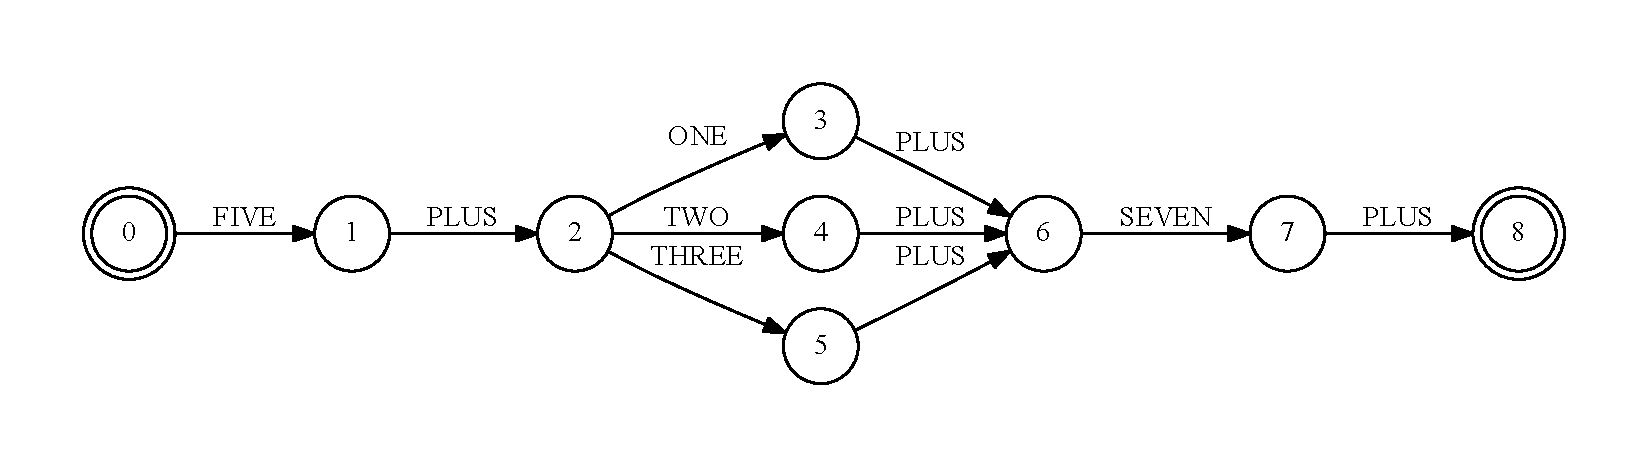
\includegraphics[width=\textwidth]{Azimov/pictures/block_black.pdf}
 \caption{Базовый блок при $height=3, errorBranches=0$}
 \label{block}
\end{figure}

\begin{figure}[h!]
 \centering
 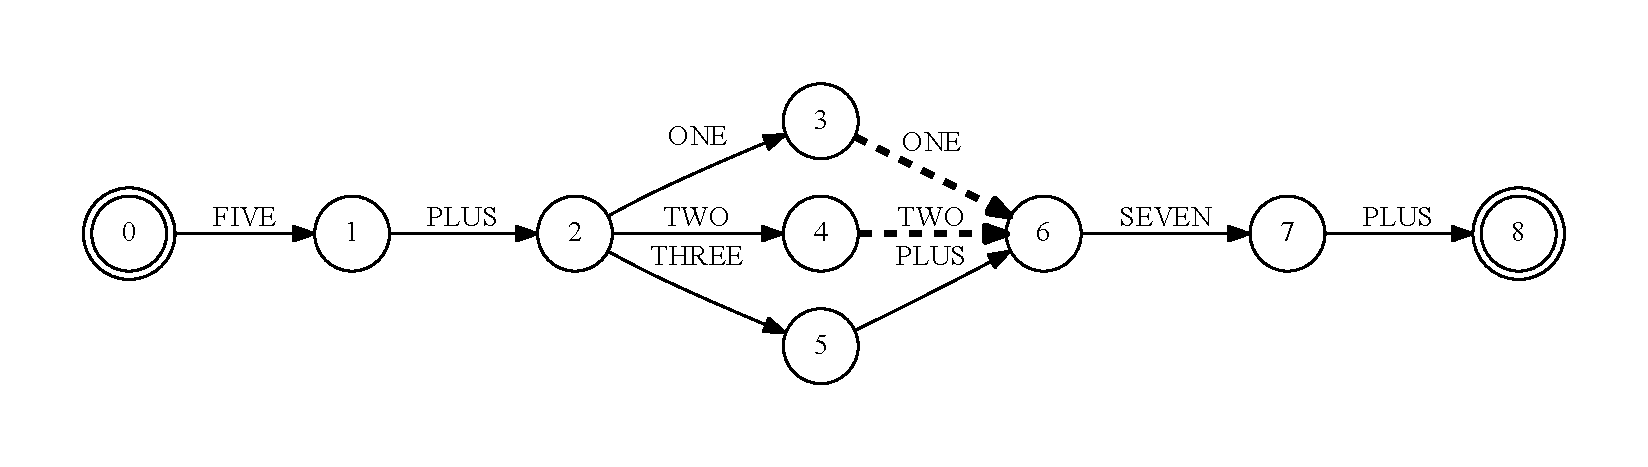
\includegraphics[width=\textwidth]{Azimov/pictures/errorBlock_black.pdf}
 \caption{Базовый блок при $height=3, errorBranches=2$}
 \label{errorBlock}
\end{figure}

Замеры времени работы алгоритмов проводились на машине со следующими техническими характеристиками: Intel(R) Core(TM) i7-3630QM CPU @ 2.40GHz, RAM: 8.0~GB, процессор x64.

\begin{figure}[H]
 \centering
 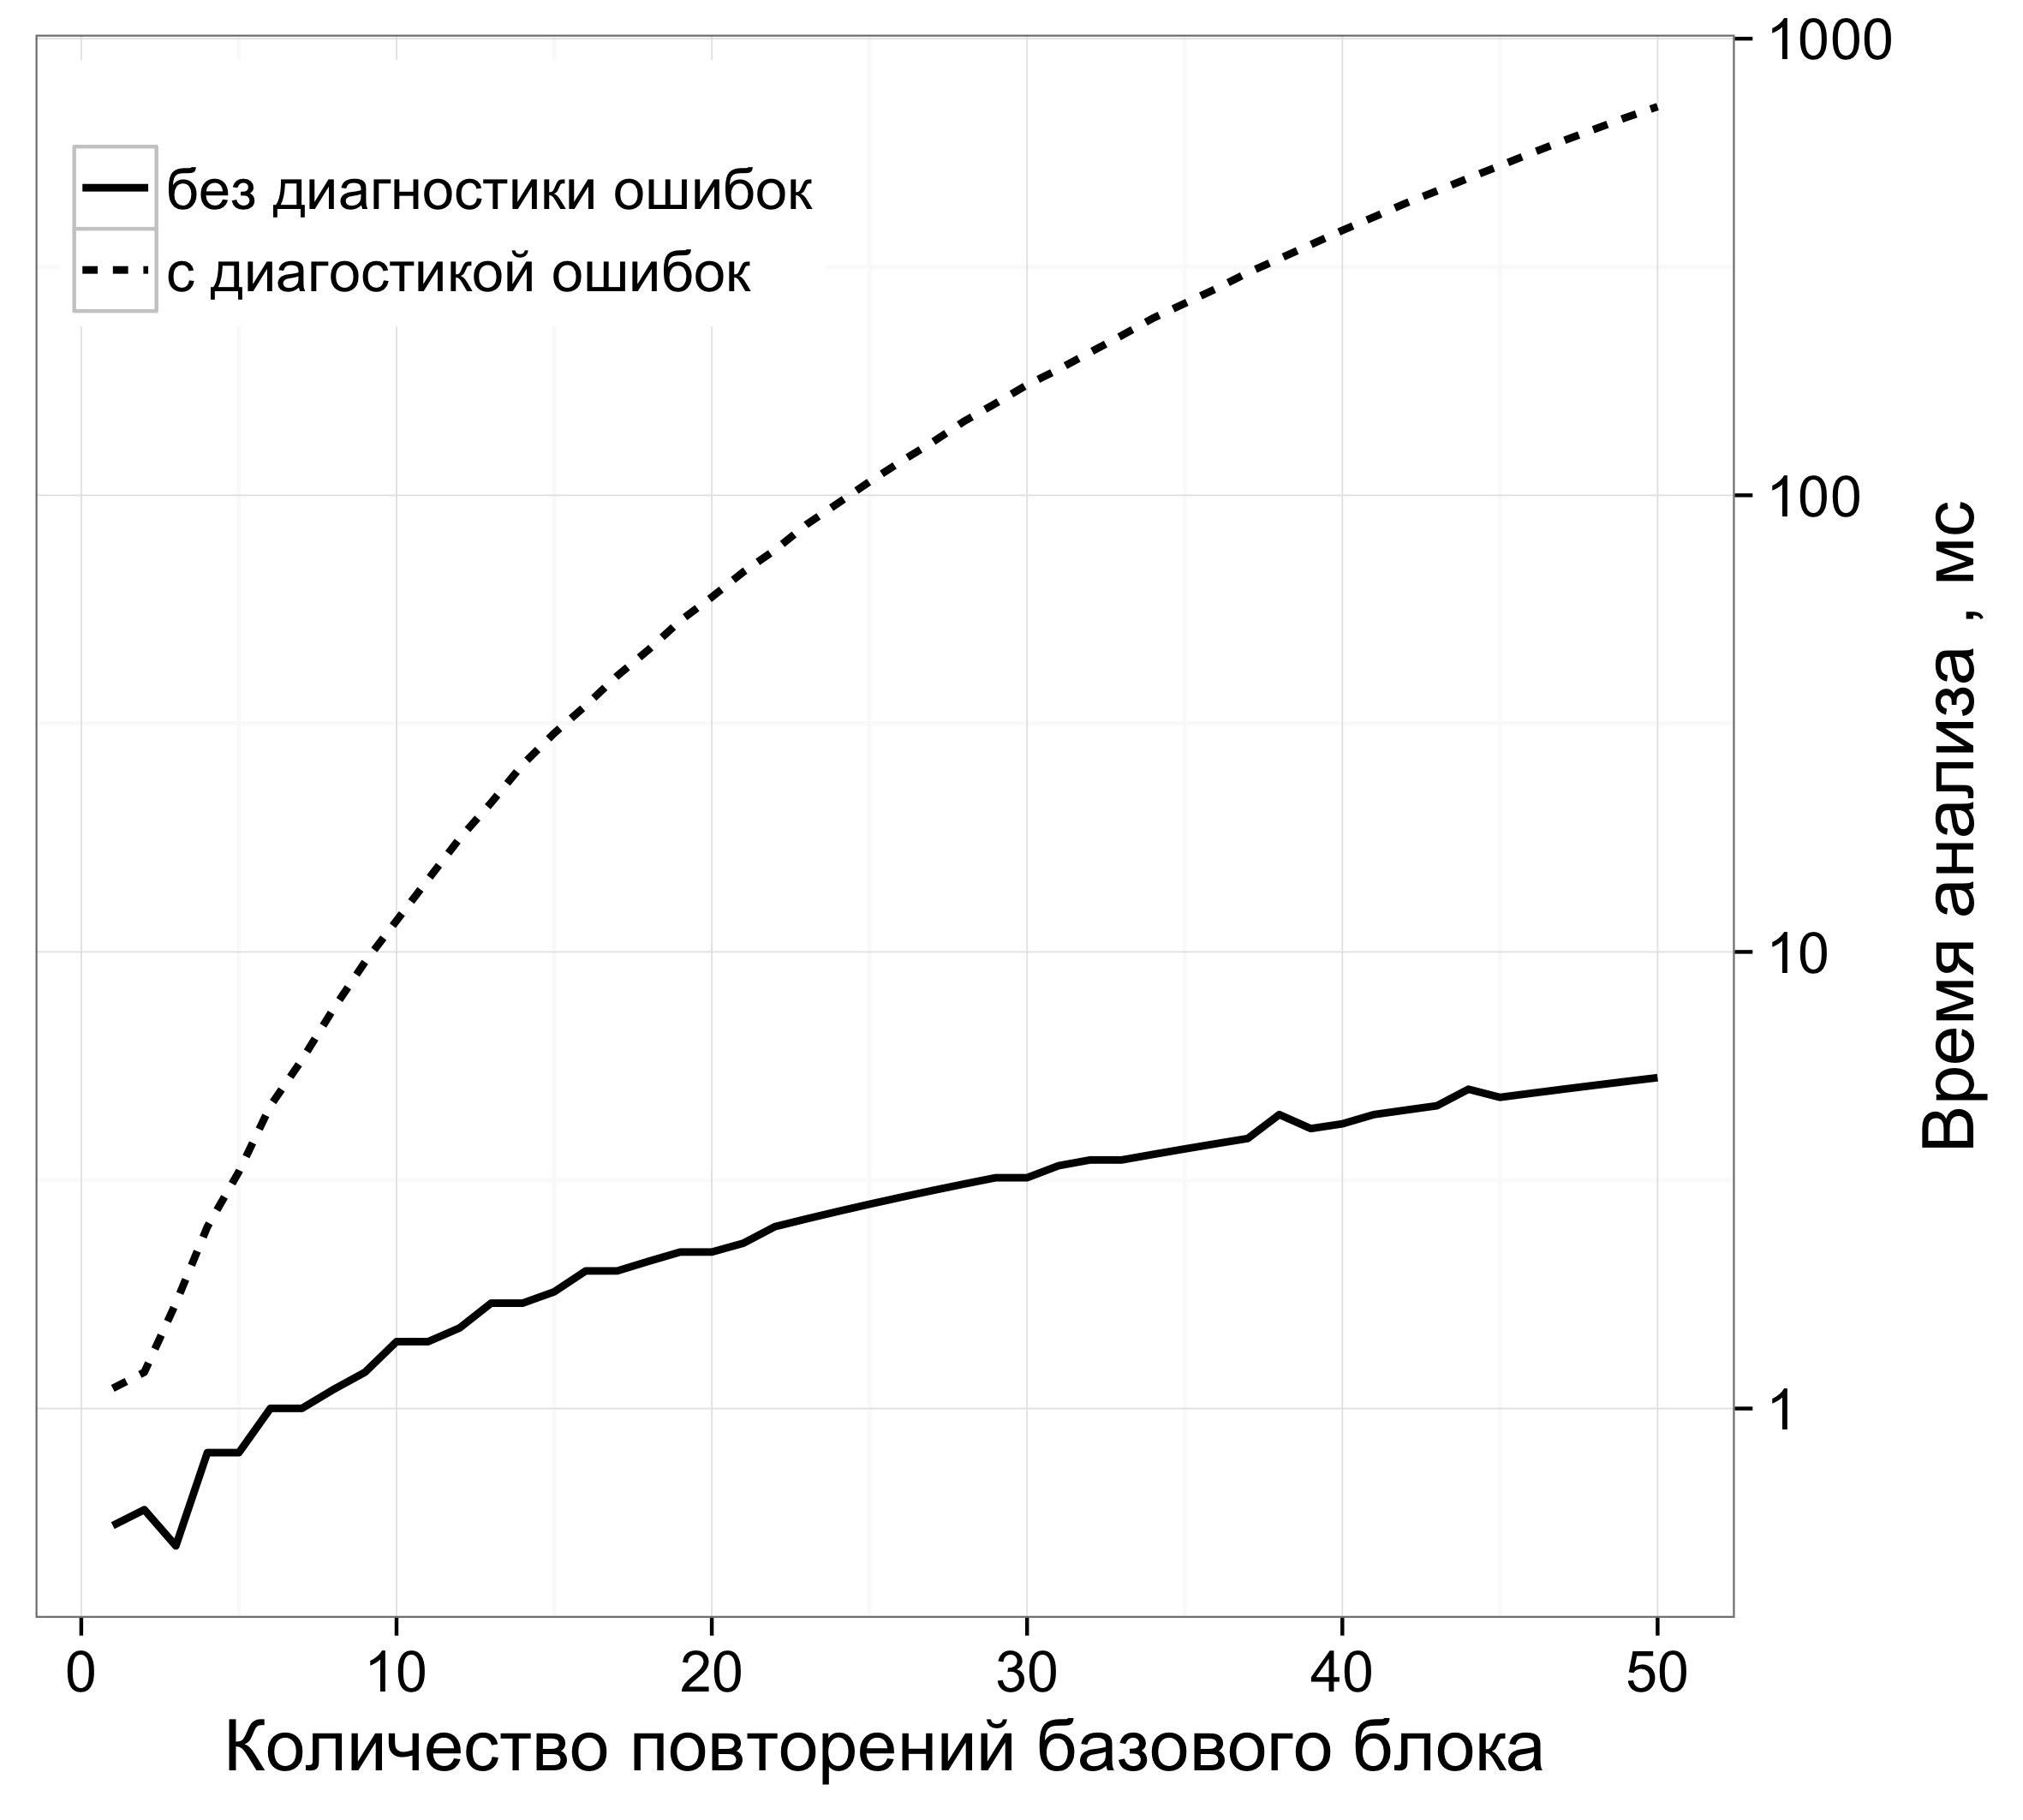
\includegraphics[width=0.9\textwidth]{Azimov/pictures/compare_black.png}
 \caption{Сравнение времени работы алгоритма синтаксического анализа до и после модификаций, при $height=4, errors=0$}
 \label{compare}
\end{figure}


Каждая серия объединяет набор из 50 тестов, каждый из которых содержит одинаковое количество ветвлений в базовом блоке, при этом количество повторений блока совпадает с порядковым номером теста ($length = i$, для теста с номером $i$). Для каждого теста измерялось время, затраченное на синтаксический анализ. Измерения проводились 10 раз, после чего усреднялись. График, представленный на рис.~\ref{compare}, иллюстрирует сравнение времени работы алгоритма синтаксического анализа до и после модификаций. Можно заметить, что выполненная модификация существенно увеличивает продолжительность анализа. Причина этого в том, что выполненная модификация является прототипом, а в будущем планируется улучшить производительность путем улучшения реализации. График на рис.~\ref{withErrors} демонстрирует зависимость времени работы модифицированного алгоритма от количества повторений базового блока и количества веток, содержащих ошибочное ребро, в каждом из них. Наблюдается уменьшение времени работы модифицированного алгоритма при увеличении количества ошибочных ребер. Одной из причин этого является уменьшение количества корректных префиксов внутреннего графа при увеличении количества ошибочных ребер.

\begin{figure}[H]
 \centering
 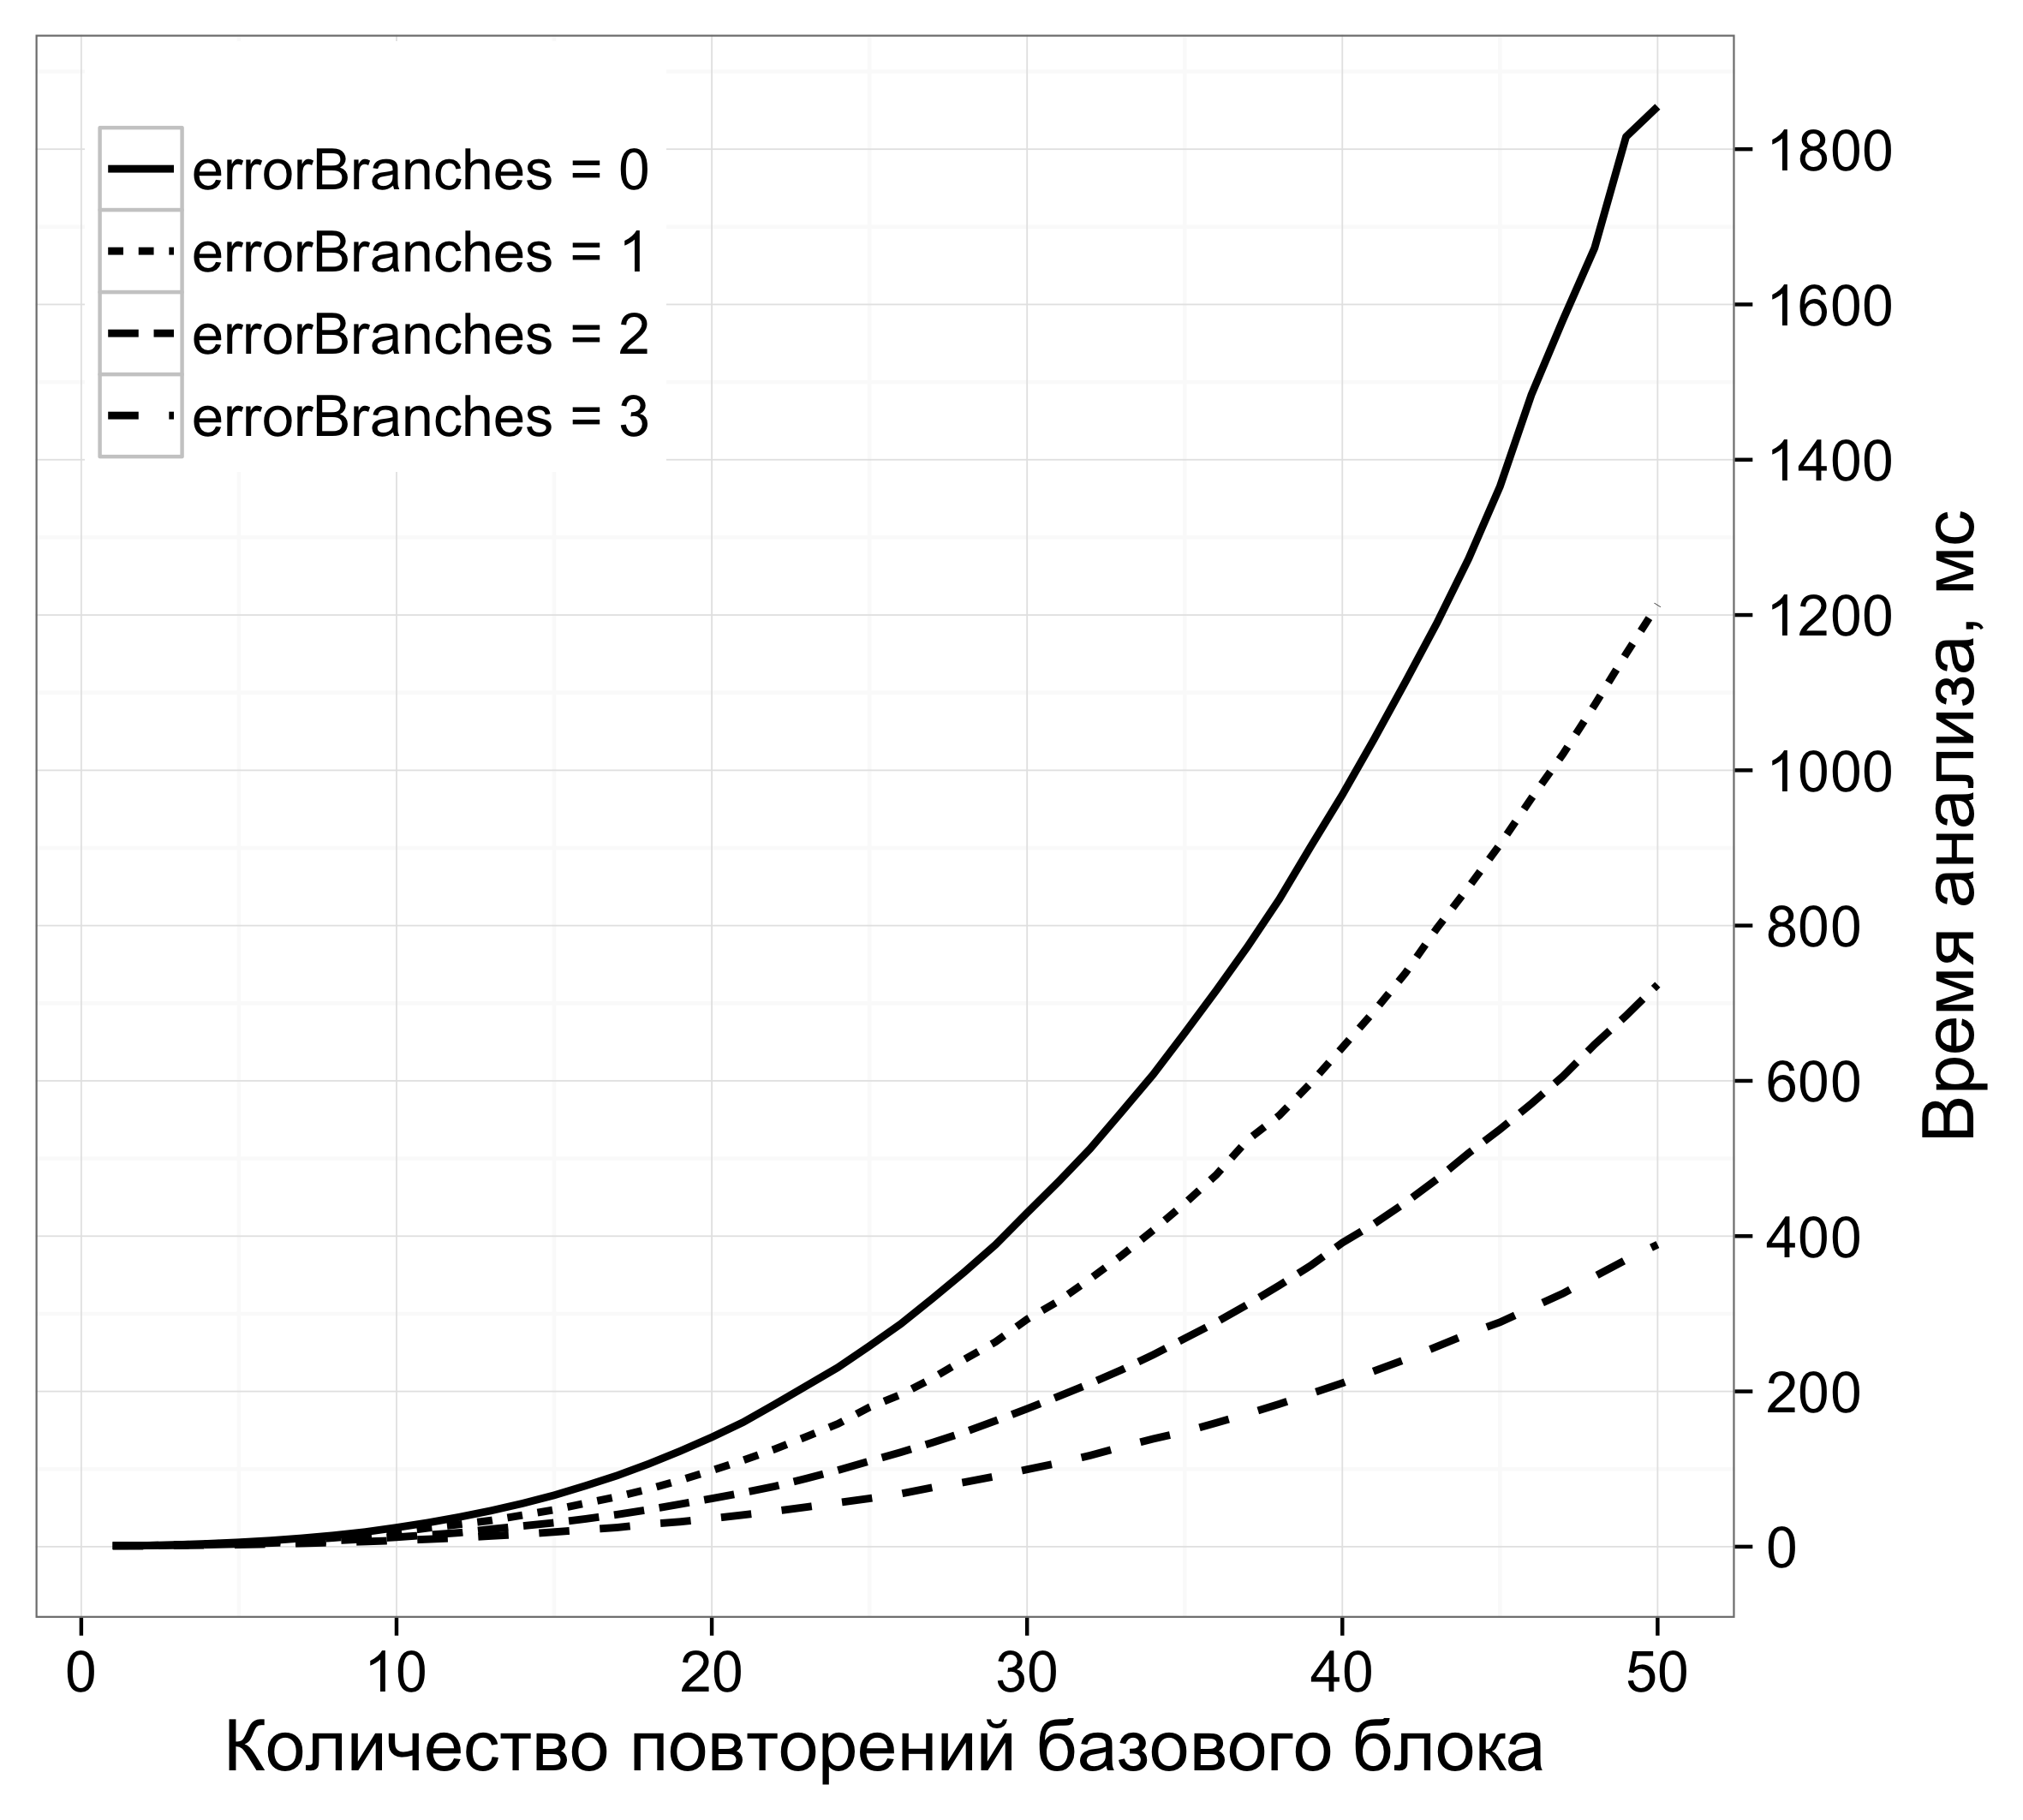
\includegraphics[width=0.9\textwidth]{Azimov/pictures/error_branches4_black.png}
 \caption{Зависимость времени работы модифицированного алгоритма от размера входного графа и количества ошибочных ребер при $height=6$}
 \label{withErrors}
\end{figure}

\section{Заключение}

В данной работе описан подход к композициональному символьному исполнению без раскрутки. Была предложена концепция композициональной памяти с символьной адресацией. Был доказан некоторый набор свойств КСП, дающий основание для подхода в стиле систем переписывания, где символьные кучи могут сами выступать как символы. Это даёт возможность автоматически порождать уравнения на состояния, решения которых в точности отражают поведения функций, работающих с динамической памятью. Было показано как свести задачу решения уравнений на состояния к задаче проверки безопасности чистых функций второго порядка.

Данная работа нацелена на теоретические основания композиционального анализа динамической памяти. Мы оставляем апробацию этого подхода на будущее. Другим направлением будущих исследований может быть расширение нашего формализма на композициональный анализ параллельных программ.

\clearpage
\setmonofont[Mapping=tex-text]{CMU Typewriter Text}
\bibliographystyle{ugost2008ls}
\bibliography{diploma.bib}
\end{document}
